\section{Event selection}
\label{selection}

\subsection{Triggers}
The events are required to pass different triggers in each channel. Standard CMS electron and muon triggers are not designed for displaced objects, so we use nonstandard triggers for both electrons and muons. For muons, we remove all trigger requirements relating to the muon transverse or longitudinal impact parameter or the vertex from which the muon originates. For electrons, we actually use photon triggers, which collect events with electrons as well as photons but do not rely on any tracking information.

In the $\Pe\Pgm$ channel, 2016 data and corresponding MC simulation events are required to pass the logical OR of two HLT paths (\longvar{HLT_Mu38NoFiltersNoVtx_Photon38_CaloIdL_v*} OR \longvar{HLT_Mu28NoFiltersNoVtxDisplaced_Photon28_CaloIdL_v*}) that were both designed for this analysis. These triggers require at least one L3 muon with $\pt>38(28)\si{\GeV}$ without any constraints on the vertex or upper bound on the transverse or longitudinal impact parameter. The second trigger requires that the absolute value of the L3 muon transverse impact parameter is greater than 0.01\unit{cm}. Each of these two triggers also requires at least one photon with loose calorimeter ID and $\ET>38(28)\si{\GeV}$. The HLT paths are seeded by \longvar{L1\_Mu5\_EG20 OR L1\_Mu20\_EG15}. The signal efficiency with these dedicated triggers is significantly higher than that of standard muon-photon HLT paths.
\fxnote{define/cite L3, ET and such?}

2017 and 2018 data and corresponding MC simulation events in the $\Pe\Pgm$ channel are required to pass \longvar{HLT_Mu43NoFiltersNoVtx_Photon43_CaloIdL_v*}. The muon \pt and photon \ET thresholds were raised with respect to 2016 due to increased pileup. Unlike in 2016, the version of this trigger that requires displaced muons was not available.

In the $\Pe\Pe$ channel, 2016 data and corresponding MC simulation events are required to pass the logical OR of two HLT paths (\longvar{HLT_Diphoton30_18_R9Id_OR_IsoCaloId_AND_HE_R9Id_Mass90_v*} OR  \longvar{HLT_DoublePhoton60_v*}). The first requires a leading photon with $\ET>30\GeV$ and a subleading photon with $\ET>\SI{18}{\GeV}$. Calorimeter identification, isolation, $H/E$, and $R_9$ requirements are made on both photons, and the diphoton invariant mass must be $>\SI{90}{\GeV}$. This HLT path is seeded by a suite of single-photon and double-photon L1 seeds. This path is highly efficient at low $\PSQt$ mass. The second trigger simply requires at least two photons with $\ET>\SI{60}{\GeV}$. This HLT path is seeded by a suite of nonisolated single-photon, double-photon, single-jet, and single-tau-jet L1 seeds. This path is highly efficient at large $\PSQt$ mass and lifetime.
\fxnote{define H/E and such}

2017 and 2018 data and corresponding MC simulation events are required to pass \longvar{HLT_Diphoton30_22_R9Id_OR_IsoCaloId_AND_HE_R9Id_Mass90_v*} OR  \longvar{HLT_DoublePhoton70_v*}. The photon \ET thresholds were raised with respect to 2016 due to increased pileup.

In the $\Pgm\Pgm$ channel, 2016 data and corresponding MC simulation events are required to pass the logical OR of two HLT paths (\longvar{HLT_DoubleMu33NoFiltersNoVtx_v*} OR \longvar{HLT_DoubleMu23NoFiltersNoVtxDisplaced_v*}) that were both designed for this analysis. These triggers require at least two L3 muons with $\pt>33(23)\si{\GeV}$ without any constraints on the vertex or upper bound on the transverse or longitudinal impact parameter. The second trigger requires that the L3 muon transverse impact parameter is greater than 0.01~\unit{cm}. The HLT paths are seeded by the lowest \pt threshold unprescaled double-muon L1 seeds. The signal efficiency with these dedicated triggers is significantly higher than that of standard dimuon HLT paths.

2017 and 2018 data and corresponding MC simulation events are required to pass \longvar{HLT_DoubleMu43NoFiltersNoVtx_v*}. The muon \pt threshold was raised with respect to 2016 due to increased pileup. Unlike in 2016, the version of this trigger that requires displaced muons was not available.


\subsection{Preselection}
\label{preselection}
Starting from the events collected with the triggers described above, we next apply a preselection that selects the events to be analyzed. The preselection criteria vary by channel and year, but the fundamental goal is always to select events with at least one good offline reconstructed lepton of each flavor required by the channel. 

The preselection selects events with at least one good particle flow (PF) electron and at least one good global PF muon ~\cite{cms_pf} in the $\Pe\Pgm$ channel, events with at least two good PF electrons in the $\Pe\Pe$ channel, and events with at least two good global PF muons in the $\Pgm\Pgm$ channel.  We set requirements on these electrons and muons as shown in Tables~\ref{preselection_emu}, ~\ref{preselection_ee}, and ~\ref{preselection_mumu}. The electron and muon \pt  requirements are chosen to be in the plateau of the trigger turn-on curve, and electron and muon $\abs{\eta}$ requirements are chosen to remove leptons with poorly measured transverse impact parameter, which are more common at large $\abs{\eta}$ (see Appendix~\ref{large_eta} for further discussion). Electrons that traverse the gap between the endcap and barrel detectors are also rejected due to the known loss of reconstruction performance in this region. \fxnote{cite something for gap reco performance?}\fxnote{include trigg eff plots}

\begin{sidewaystable}
\noindent \centering{}
\topcaption{The $\Pe\Pgm$ preselection criteria. The electron and muon \pt thresholds increased in 2017 because the HLT electron and muon \pt thresholds increased.}
\label{preselection_emu}
\begin{tabular}{lll}
\hline
\multicolumn{3}{c}{Object-level selections}\\
Selection variable & Electron     & Muon \\
\hline 
Number             & $\geq1$         & $\geq1$\\[2mm]
\multirow{2}{*}{\pt}& $>42\GeV$ (2016)    & $>40\GeV$ (2016)\\
                & $>45\GeV$ (2017 and 2018)    & $>45\GeV$ (2017 and 2018)\\[2mm]
$\abs{\eta}$           & $<1.5$      & $<1.5$\\[2mm]
 & not in ECAL gap & -\\[2mm]
\multirow{2}{*}{$\eta-\phi$ (pixel power supply issue)}& veto ($1.0<\eta<1.5$ and $\phi>2.7$) (2017)    & veto ($1.0<\eta<1.5$ and $\phi>2.7$) (2017)\\
                & veto ($0.3<\eta<1.2$ and $0.4<\phi<0.8$) (2018)   & veto ($0.3<\eta<1.2$ and $0.4<\phi<0.8$) (2018)\\[2mm]
ID                 & Tight (cut-based) & Tight (cut-based)\\[2mm]
Custom isolation   & Tight        & Tight \\
\hline
\hline
\multicolumn{3}{c}{Event-level selections}\\
\hline
\multicolumn{3}{c}{Zero $\Pgm\Pgm$ pairs with $\cos{\alpha}<-0.99$} \\
\multicolumn{3}{c}{Reject $\Delta t<-20\ns$, if both timing ndof$>7$} \\
\multicolumn{3}{c}{At least one $\Pe\Pgm$ pair with $\DR(\Pe,\Pgm)>0.2$} \\
\multicolumn{3}{c}{Reject events where the candidate electron and muon form a good displaced vertex that overlaps with the tracker material} \\
\hline
\end{tabular}
\end{sidewaystable}
\begin{sidewaystable}
\setlength{\tabcolsep}{40pt}
\noindent \centering{}
\topcaption{The $\Pe\Pe$ preselection criteria. The electron \pt threshold increase in 2017 and 2018 in accordance with the increased HLT electron \pt threshold.}
\label{preselection_ee}
\begin{tabular}{ll}
\hline
\multicolumn{2}{c}{Object-level selections}\\
Selection variable & Electron          \\
\hline
Number               & $\geq2$              \\[2mm]
\multirow{2}{*}{\pt} & $>65\GeV$ (2016)\\
                     & $>75\GeV$ (2017 and 2018)\\[2mm]
$\abs{\eta}$             & $<1.5$\\[2mm]
                     & not in ECAL gap\\[2mm]
\multirow{2}{*}{$\eta-\phi$ (pixel power supply issue)}& veto ($1.0<\eta<1.5$ and $\phi>2.7$) (2017)\\
                & veto ($0.3<\eta<1.2$ and $0.4<\phi<0.8$) (2018)\\[2mm]
ID                   & Tight (cut-based) \\[2mm]
Custom isolation     & Tight             \\
\hline
\hline
\multicolumn{2}{c}{Event-level selections}\\
\hline
\multicolumn{2}{c}{At least one $\Pe\Pe$ pair with $\DR(\Pe,\Pe)>0.2$} \\
\multicolumn{2}{c}{Reject events with candidate leptons form a displaced vertex in the tracker material} \\
\multicolumn{2}{c}{Reject events with displaced muons in the $\Pe\Pgm$ channel inclusive signal region} \\
\hline
\end{tabular}
\end{sidewaystable}
\begin{sidewaystable}
\setlength{\tabcolsep}{40pt}
\noindent \centering{}
\topcaption{The $\Pgm\Pgm$ preselection criteria. The muon \pt threshold increases in 2017 and 2018 in accordance with the increased HLT muon \pt threshold.}
\label{preselection_mumu}
\begin{tabular}{ll}
\hline
\multicolumn{2}{c}{Object-level selections}\\
Selection variable & Muon          \\
\hline
Number               & $\geq2$              \\[2mm]
\multirow{2}{*}{\pt} & $>35\GeV$ (2016) \\
                     & $>45\GeV$ (2017 and 2018) \\[2mm]
$\abs{\eta}$             & $<1.5$            \\[2mm]
\multirow{2}{*}{$\eta-\phi$ (pixel power supply issue)}& veto ($1.0<\eta<1.5$ and $\phi>2.7$) (2017)\\
                & veto ($0.3<\eta<1.2$ and $0.4<\phi<0.8$) (2018)\\[2mm]
ID                   & Tight (cut-based) \\[2mm]
Custom isolation     & Tight             \\
\hline
\hline
\multicolumn{2}{c}{Event-level selections}\\
\hline
\multicolumn{2}{c}{Zero $\Pgm\Pgm$ pairs with $\cos{\alpha}<-0.99$} \\
\multicolumn{2}{c}{Reject $\Delta t<-20\ns$, if both timing ndof$>7$} \\
\multicolumn{2}{c}{At least one $\Pgm\Pgm$ pair with $\DR(\Pgm,\Pgm)>0.2$} \\
\multicolumn{2}{c}{Reject events with candidate leptons form a displaced vertex in the tracker material} \\
\multicolumn{2}{c}{Reject events with displaced electrons in the $\Pe\Pgm$ channel inclusive signal region} \\
\hline
\end{tabular}
\end{sidewaystable}

We use tight cut-based identification (ID) on the electrons and muons to select well-reconstructed leptons, but unlike the standard ID definitions used in many CMS analyses, we do not place any requirements on the transverse and longitudinal impact parameters. For electrons, the ID corresponds to the \longvar{egmGsfElectronIDs:cutBasedElectronID-Summer16-80X-V1-tight} in 2016, \longvar{egmGsfElectronIDs:cutBasedElectronID-Fall17-94X-V1-tight} in 2017, and \longvar{egmGsfElectronIDs:cutBasedElectronID-Fall17-94X-V2-tight} in 2018~\cite{egammaPOGtightID}. The electron and muon tight ID requirements are summarized in Tables \ref{e_tight_id} and \ref{tab:mu_tight_id}.

\begin{table}
\noindent \centering{}
\topcaption{The electron tight ID requirements, which are identical to the tight cut-based ID from the CMS EGamma Physics Object Group with the $d_0$ and longitudinal impact parameter requirements removed.\fxnote{cite something to define quantities}}
\label{e_tight_id}
\begin{tabular}{ll}
\hline
Electron ID requirements\\
\hline 
\multirow{2}{*}{full5x5 $\sigma I \eta I\eta <$}     & 0.0104 (2018, 2017)                \\
                                                     & 0.00998 (2016)                     \\[2mm]
\multirow{3}{*}{$|\delta\eta \mathrm{Seed}| < $}     & 0.00255 (2018)                     \\
                                                     & 0.00353 (2017)                     \\
                                                     & 0.00308 (2016)                     \\[2mm]
\multirow{3}{*}{$|\delta\phi \mathrm{In}| < $}       & 0.022 (2018)                       \\
                                                     & 0.0499 (2017)                      \\
                                                     & 0.0816 (2016)                      \\[2mm]
\multirow{3}{*}{$\mathrm{H/E} <$}                    & $0.026+1.15/\mathrm{E}+0.0324\rho/\mathrm{E}$ (2018)  \\
& $0.026+1.12/\mathrm{E}+0.0368\rho/\mathrm{E}$ (2017)  \\
& 0.0414 (2016)  \\[2mm]
\multirow{3}{*}{Rel. comb. PF iso with EA corr $<$}  & $0.0287+0.506/\pt$ (2018)         \\
                                                     & 0.0361 (2017)          \\
                                                     & 0.0588 (2016)          \\[2mm]
\multirow{3}{*}{$|1/\mathrm{E}-1/\mathrm{p}|<$}   & 0.159 (2018)              \\
                                                  & 0.0278 (2017)             \\
                                                  & 0.0129 (2016)             \\[2mm]
expected missing inner hits $<=$ & 1                            \\[2mm]
pass conversion veto	         & yes                          \\[2mm]
\hline
\end{tabular}
\end{table}
\begin{table}
\noindent \centering{}
\topcaption{The muon tight ID requirements, which are identical to the tight cut-based ID from the CMS Muon Physics Object Group with the requirements on $d_0$ and $d_z$ removed.}
\label{tab:mu_tight_id}
\begin{tabular}{ll}
\hline
Muon ID requirements\\
\hline 
Is a global muon\\
Is a PF muon\\
$\chi^{2}/\mathrm{n_{dof}}$ of the global-muon track fit is $<10$\\
At least one muon-chamber hit included in the global-muon track fit\\
Muon segments in at least two muon stations\\
At least 1 valid pixel hit\\
At least 6 tracker layers with hits\\
\hline
\end{tabular}
\end{table}

We require tight PF isolation on the electrons and muons. However, we use a modified isolation definition that accounts for the fact that displaced leptons may be associated with the wrong primary vertex. The standard PF isolation assumes all energy from primary vertices other than the leading primary vertex is due to pileup, which is not true when the primary vertex ordering is altered by an incorrectly associated lepton. We have therefore modified the pileup correction to be agnostic to the primary vertex ordering by allowing PF candidates from any primary vertex to contribute to the isolation sum and by using a simple $\rho$-based pileup correction, where $\rho$ is the total transverse energy of all the PF candidates divided by the total detector area. Figure~\ref{iso_pu_term_comparison} shows how the size of the pileup correction term depends on lepton displacement in the standard isolation but not in the modified isolation described here. We use the modified isolation definition for both electrons and muons while keeping the original tight working point for electrons and slightly tightening the tight working point for muons. In the end, we require that the relative isolation is $<0.10$ for muons and $<0.0588$ ($0.0571$) for electrons in the barrel (endcap) in 2016 and $<0.0287+0.506/\pt$ ($0.0445+0.963/\pt$) for electrons in the barrel (endcap) in 2017 and 2018. As shown in Fig.~\ref{iso_performance_comparison} and Fig.~\ref{iso_signal_bg}, this modified PF isolation rejects substantially more background when the leptons are displaced without significantly altering the signal yield. We note, however, that there may still be some minor dependence on the primary vertex selection in the PF muon requirement because the PF muon selection includes some loose isolation requirements where the charged hadron component is constrained to the selected primary vertex.

\begin{figure}
\centering
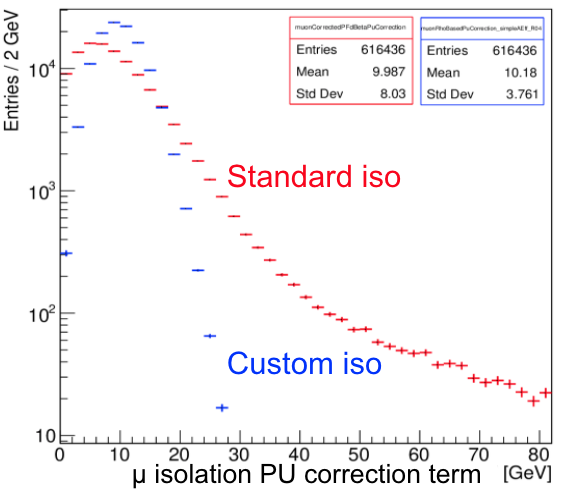
\includegraphics[width=0.44\textwidth]{figures/selection/CustomVsStandardMuIsoPUcorrection_2018emuTTbar_PCR.png}
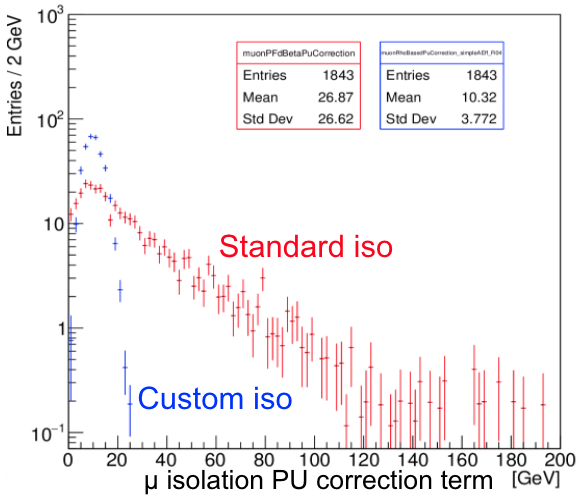
\includegraphics[width=0.45\textwidth]{figures/selection/CustomVsStandardMuIsoPUcorrection_2018emuTTbar_500To1000um.png}
\caption{The muon isolation pileup correction term, for the standard muon isolation and the modified muon isolation in simulated \ttbar events that pass the $\Pe\Pgm$ preselection in 2018 conditions. The plot on the left is for muon $\ad<\SI{100}{\um}$, and the plot on the right is for muon $500<\ad<\SI{1000}{\um}$.}
\label{iso_pu_term_comparison}
\end{figure}

\begin{figure}\fxnote{weirdly low resolution}
\centering
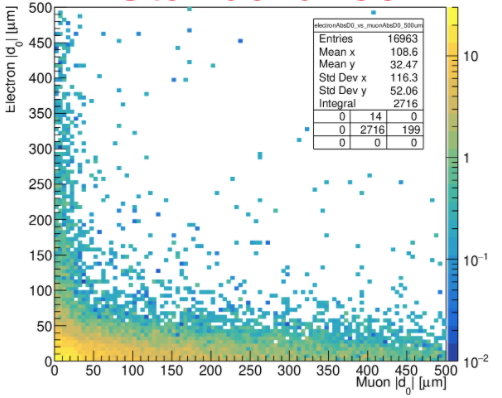
\includegraphics[width=0.45\textwidth]{figures/selection/StandardIso_ElectronD0vsMuonD0_2018emuTTbar.png}
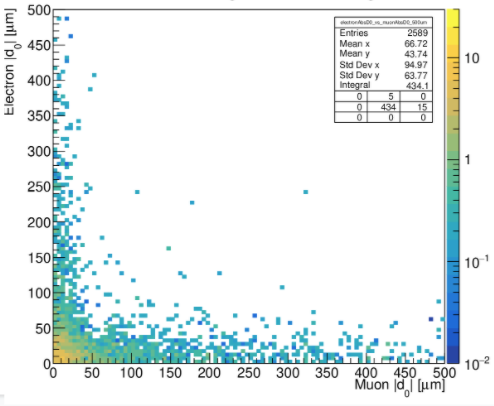
\includegraphics[width=0.44\textwidth]{figures/selection/CustomIso_ElectronD0vsMuonD0_2018emuTTbar.png}
\caption{The electron \ad versus the muon \ad, for \ttbar simulated events that pass the $\Pe\Pgm$ preselection and where at least one lepton comes from a heavy-flavor meson. The plot on the left uses the standard isolation, and the plot on the right uses the modified isolation.}
\label{iso_performance_comparison}
\end{figure}

\begin{figure}\fxnote{weirdly low resolution}
\centering
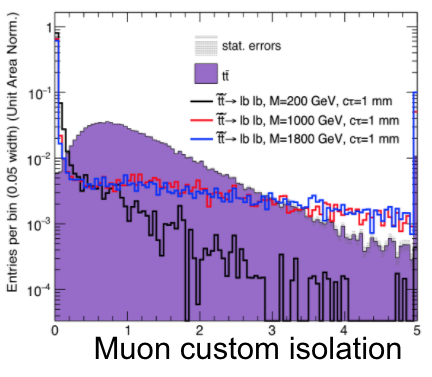
\includegraphics[width=0.5\textwidth]{figures/selection/MuonCustomIso_TTbar_Signal.png}
\caption{The muon custom isolation distribution for simulated \ttbar background and \stoptolb signal events in 2018 conditions\fxnote{specify selection}.}
\label{iso_signal_bg}
\end{figure}

We also reject electrons and muons in certain regions of the $\eta$-$\phi$ plane where lepton \ad is more likely to be mismeasured. We identify these regions as highly populated bins in the electron $\eta$-$\phi$ distribution in a prompt-muon, displaced-electron control region in 2017 and 2018 data. No such bins are present in 2016 data. The identified regions coincide with regions found by a previous CMS analysis~\cite{CMS:DisaTrack} to be affected by power supply issues in the pixel detector. The $\eta$-$\phi$ variation is more apparent for displaced electrons than displaced muons, so we use data in a prompt muon ($\ad<\SI{40}{\um}$), displaced electron ($\num{100}<\ad<\SI{500}{\um}$) control region to define the  regions used for both electrons and muons. In 2017, the rejected region is $1.0<\eta<1.5$, $\phi>2.7$, and in 2018 the rejected region is $0.3<\eta<1.2$, $0.4<\phi<0.8$.
\fxnote{include eta-phi plots}

In addition to these object-level selections, we also impose a few event-level selections designed to remove potential backgrounds from cosmic rays, material interactions, and displaced decays of SM hadrons. To remove cosmic-ray muons in the $\Pgm\Pgm$ and $\Pe\Pgm$ channels, we require there be zero pairs of muons with $\cos{\alpha}<-0.99$, where $\alpha$ is the 3D angle between the muons, and that the relative time between the leading two muons is inconsistent with the timing of cosmic-ray muons. To do this, we look at the muon time as measured at the IP from the DTs and CSCs, assuming the muons are traveling outwards from the center of the detector. We then use the muon $\phi$ measurements to determine which muon is above the other and find $\Delta t$, the time of the lower muon subtracted from the time of the upper muon. We reject events with $\Delta t< -20\ns$ if the number of degrees of freedom of the timing measurements for both muons is greater than seven. To remove leptons from decays of SM hadrons, we require that the candidate leptons not be too close together in the $\eta$-$\phi$ plane. Specifically, we find that requiring $\DR>0.2$ significantly reduces the contribution from SM hadrons without noticeably affecting the signal acceptance. To remove leptons from material interactions, we reject events in which the candidate leptons form a good displaced vertex that overlaps with the tracker material. The vertices are reconstructed with the Kalman Vertex Fitter, and a ``good'' vertex is one with $\chi^{2}/\mathrm{n_{dof}}< 20$. The tracker material map is obtained from the tracker material budget measurements~\cite{Sirunyan:2018icq,CMS-DP-2019-001}. See Section~\ref{additional_bg_checks} for tests in data that involve inverting the criteria described in this paragraph. 

Finally, to ensure that the signal regions of all three channels are orthogonal to one another, we reject events in the $\Pe\Pe$ ($\Pgm\Pgm$) channel with at least one muon (electron) that passes the $\Pe\Pgm$ channel preselection and has $\ad>\SI{100}{\um}$.

In contrast to the 2015 analysis~\cite{CMS:DisplacedEMu}, we allow for the possibility of more than one lepton of each type in a given channel and set no requirements on the charge product of the lepton pair. These changes were made at the request of several theorists, including the authors of Ref.~\cite{Evans:2016zau}.

\subsection{Prompt control region}
\label{pcr}
In order to verify the implementation of our selection and corrections to simulation (see Section~\ref{corrections}), we define a prompt control region that is dominated by SM background events. Events in each channel's prompt control region are selected by requiring that they pass all of the criteria defined in Section~\ref{preselection} as well as the requirement that the candidate leptons have $\ad<\SI{50}{\um}$. We define this region in each channel in order to check for reasonable agreement between simulated SM events and data after applying the corrections described in Section~\ref{corrections}. Some examples are shown in Figures \ref{pcr_emu_2016}, \ref{pcr_ee_2016}, and \ref{pcr_mumu_2016}, which show the \pt, $\eta$, and \ad distributions of the leptons in the $\Pe\Pgm$, $\Pe\Pe$, and $\Pgm\Pgm$ prompt control regions, respectively, for 2016 data and MC simulation. The data-driven background estimation technique employed in this analysis removes the need for exact agreement between data and simulation, but the absence of any significant discrepancies gives us confidence that we are accounting for the correct sources of prompt SM leptons and that our selection and corrections are functioning as intended.

\begin{figure}
\centering
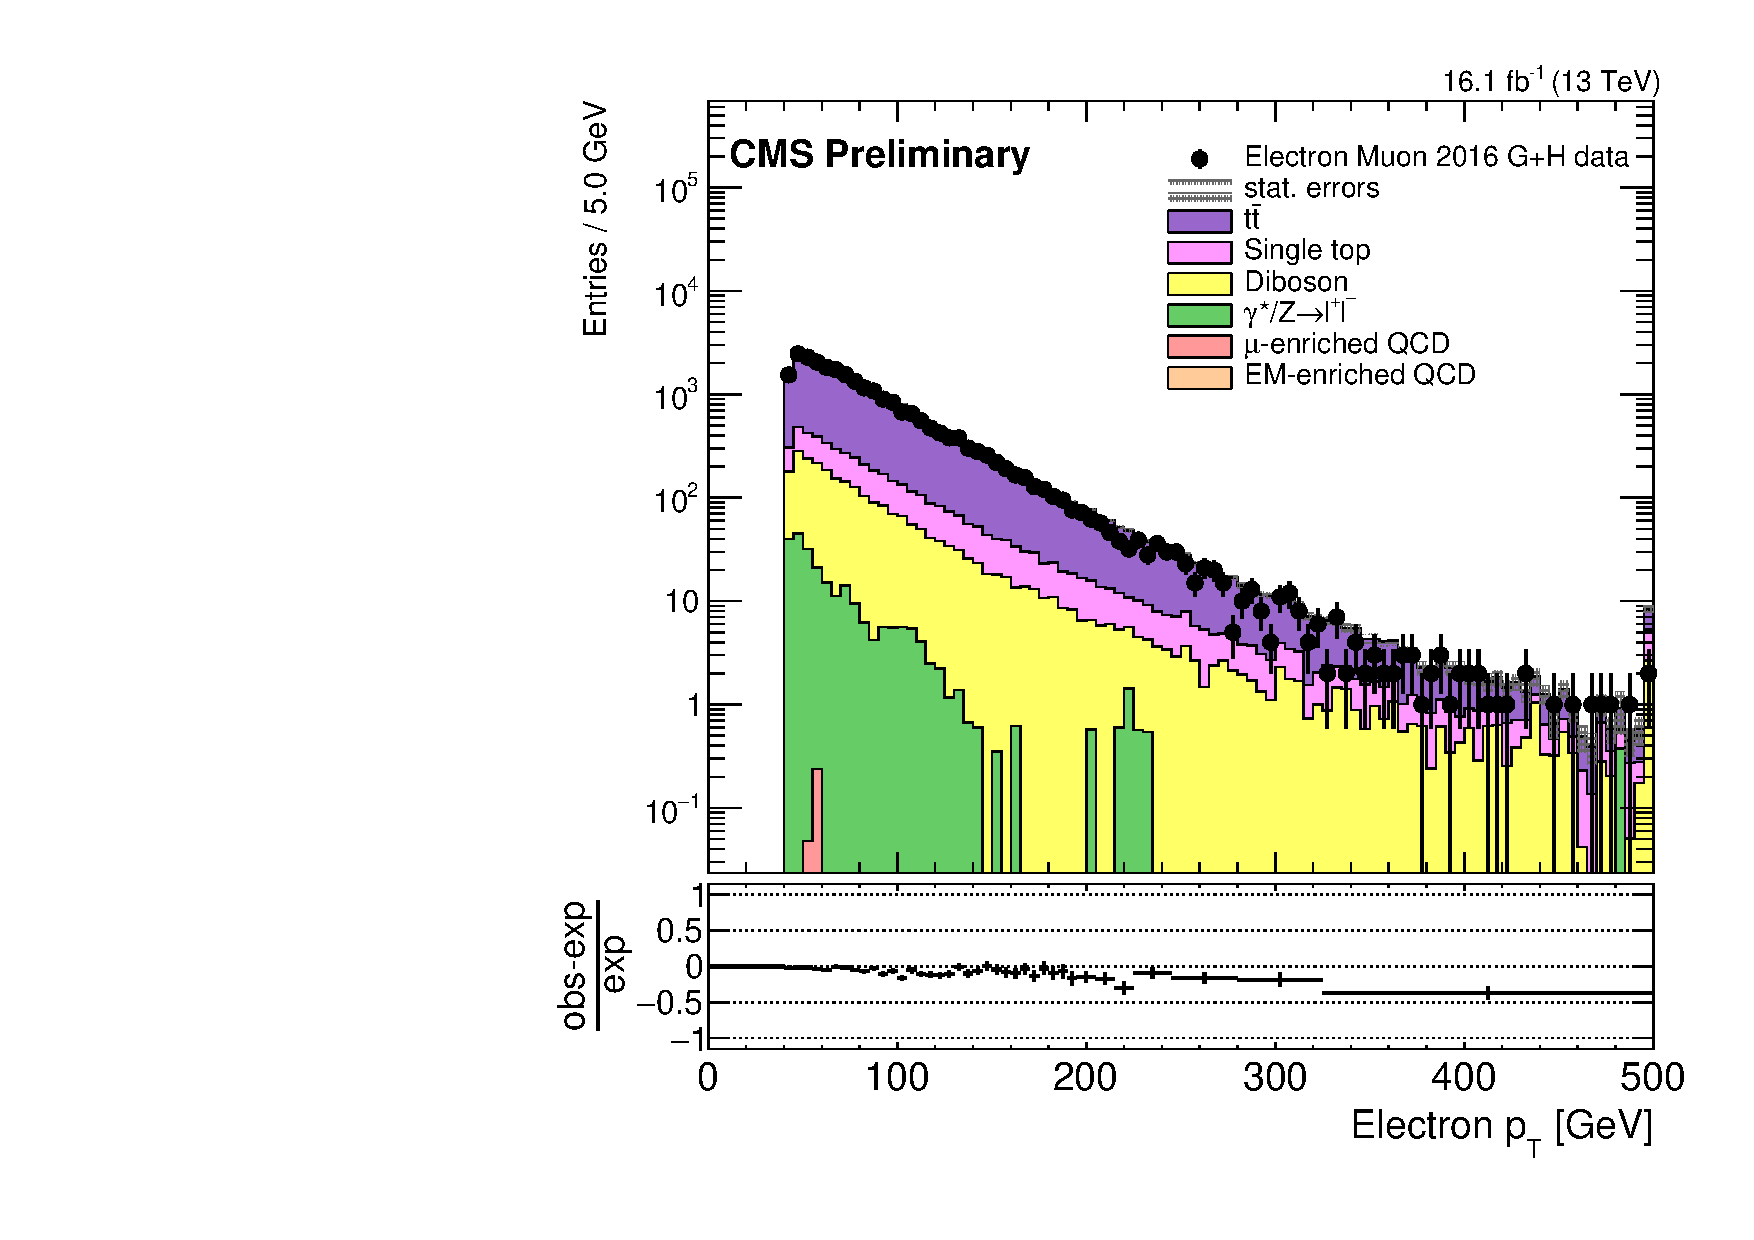
\includegraphics[width=0.3\textwidth]{figures/selection/pcr_emu_2016/electronPt.pdf}
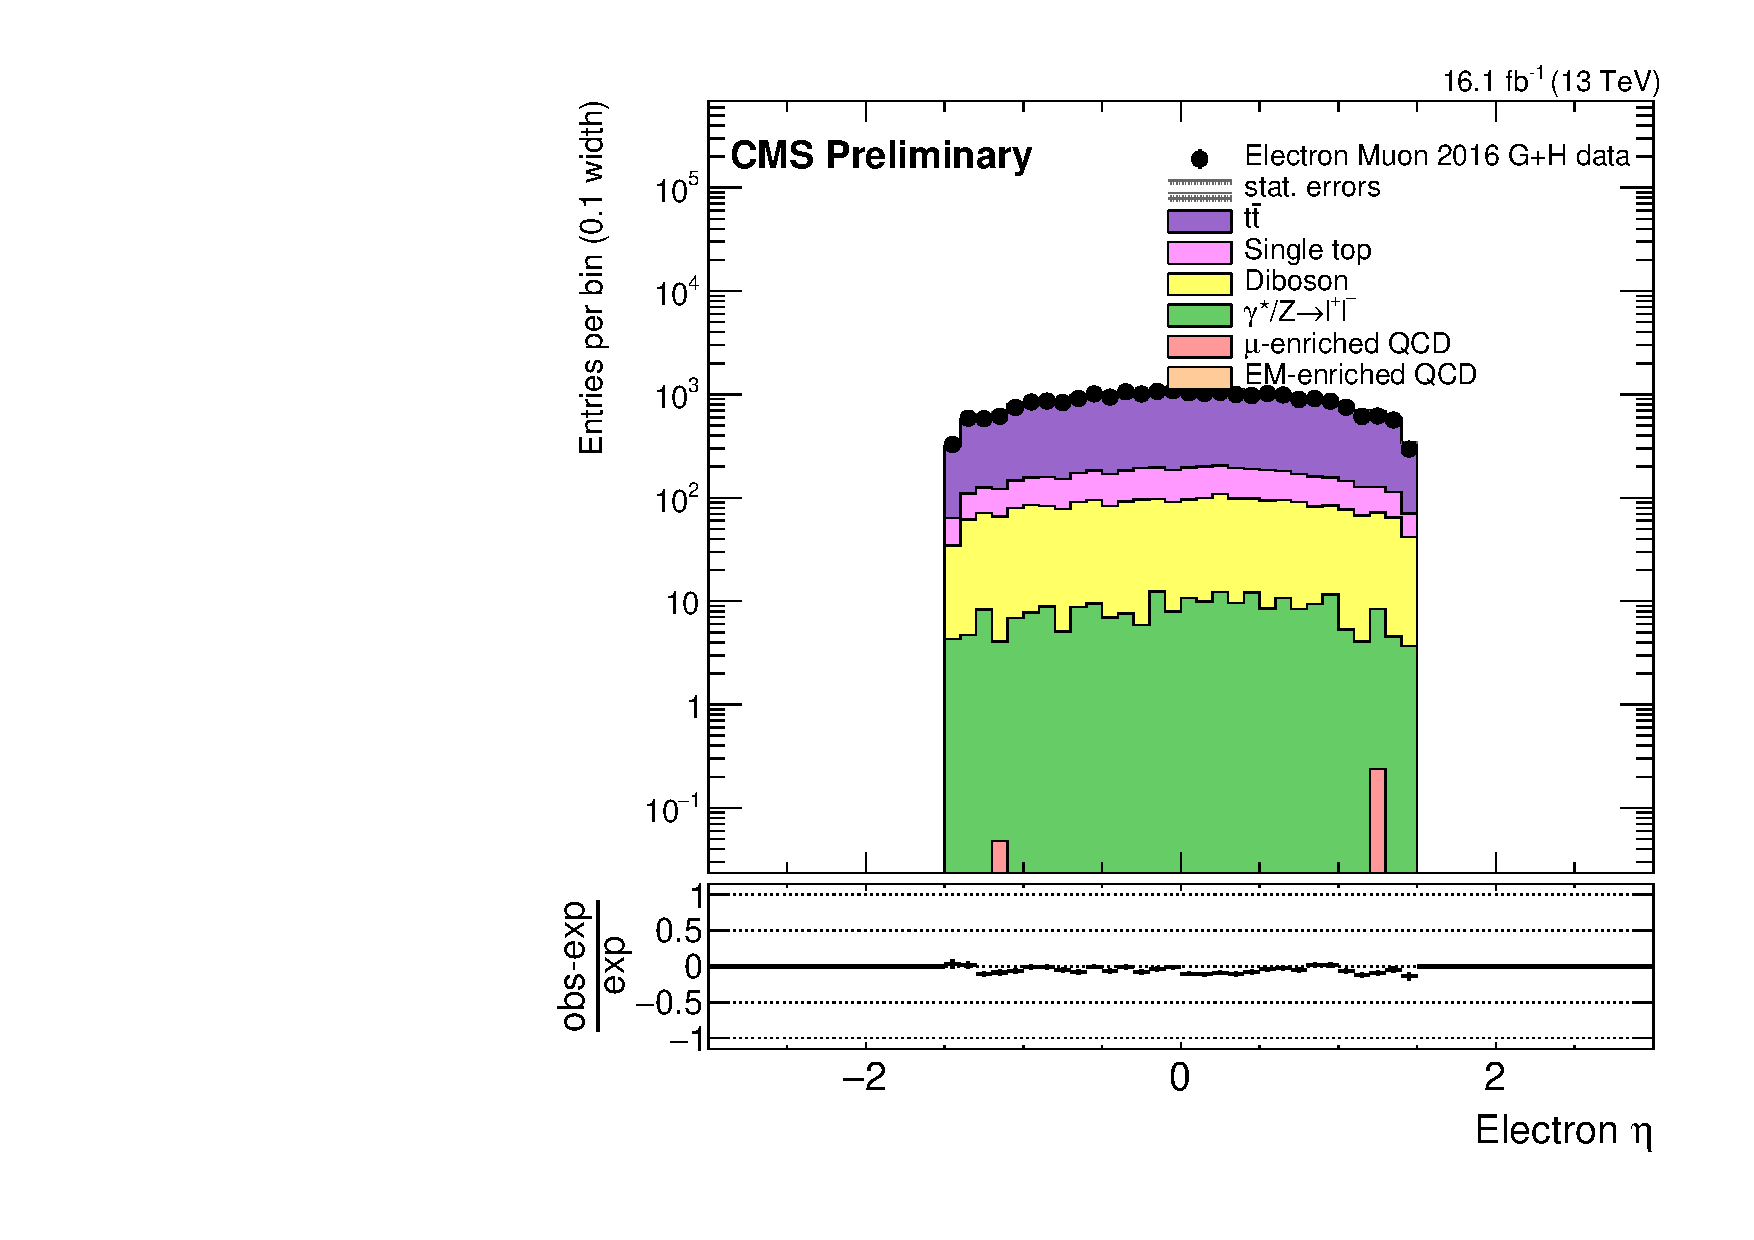
\includegraphics[width=0.3\textwidth]{figures/selection/pcr_emu_2016/electronEta.pdf}
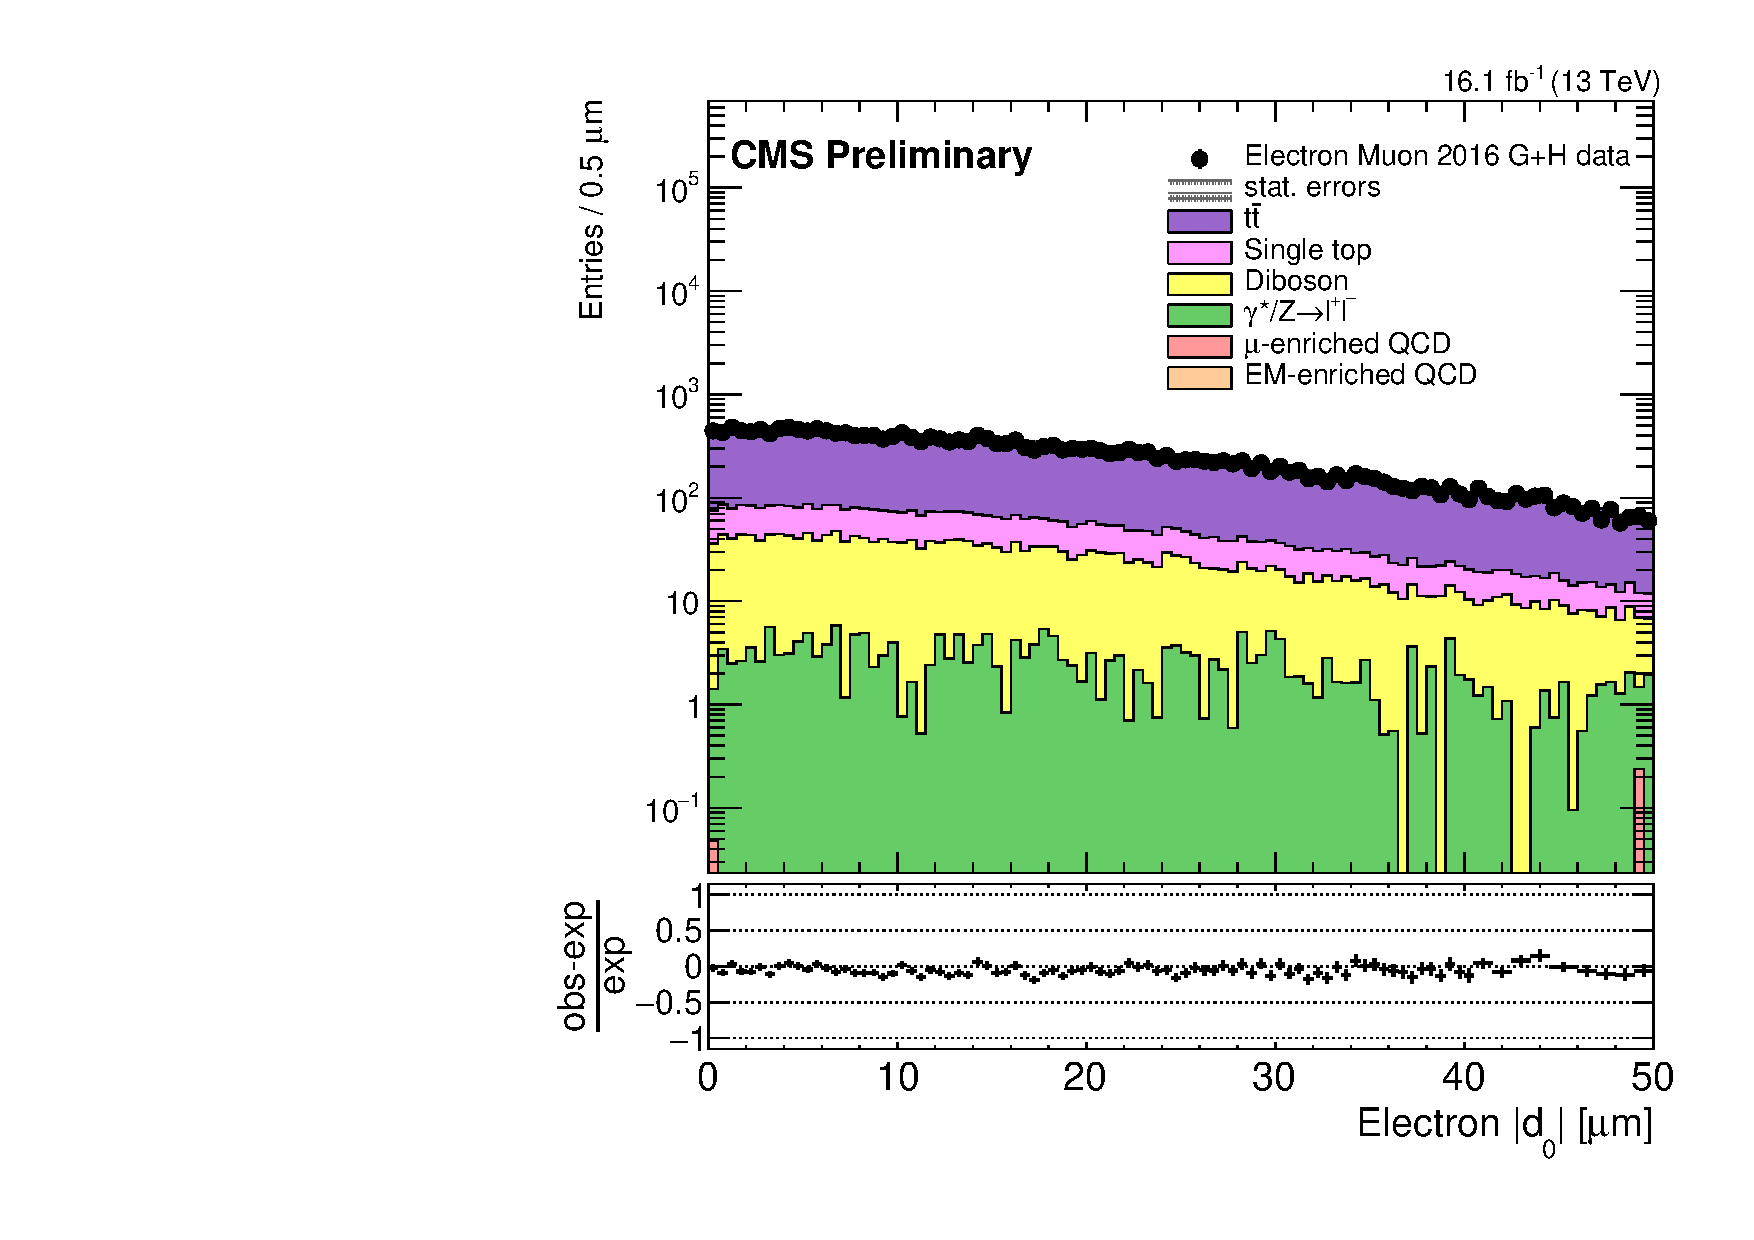
\includegraphics[width=0.3\textwidth]{figures/selection/pcr_emu_2016/electronAbsD0_50um.pdf}
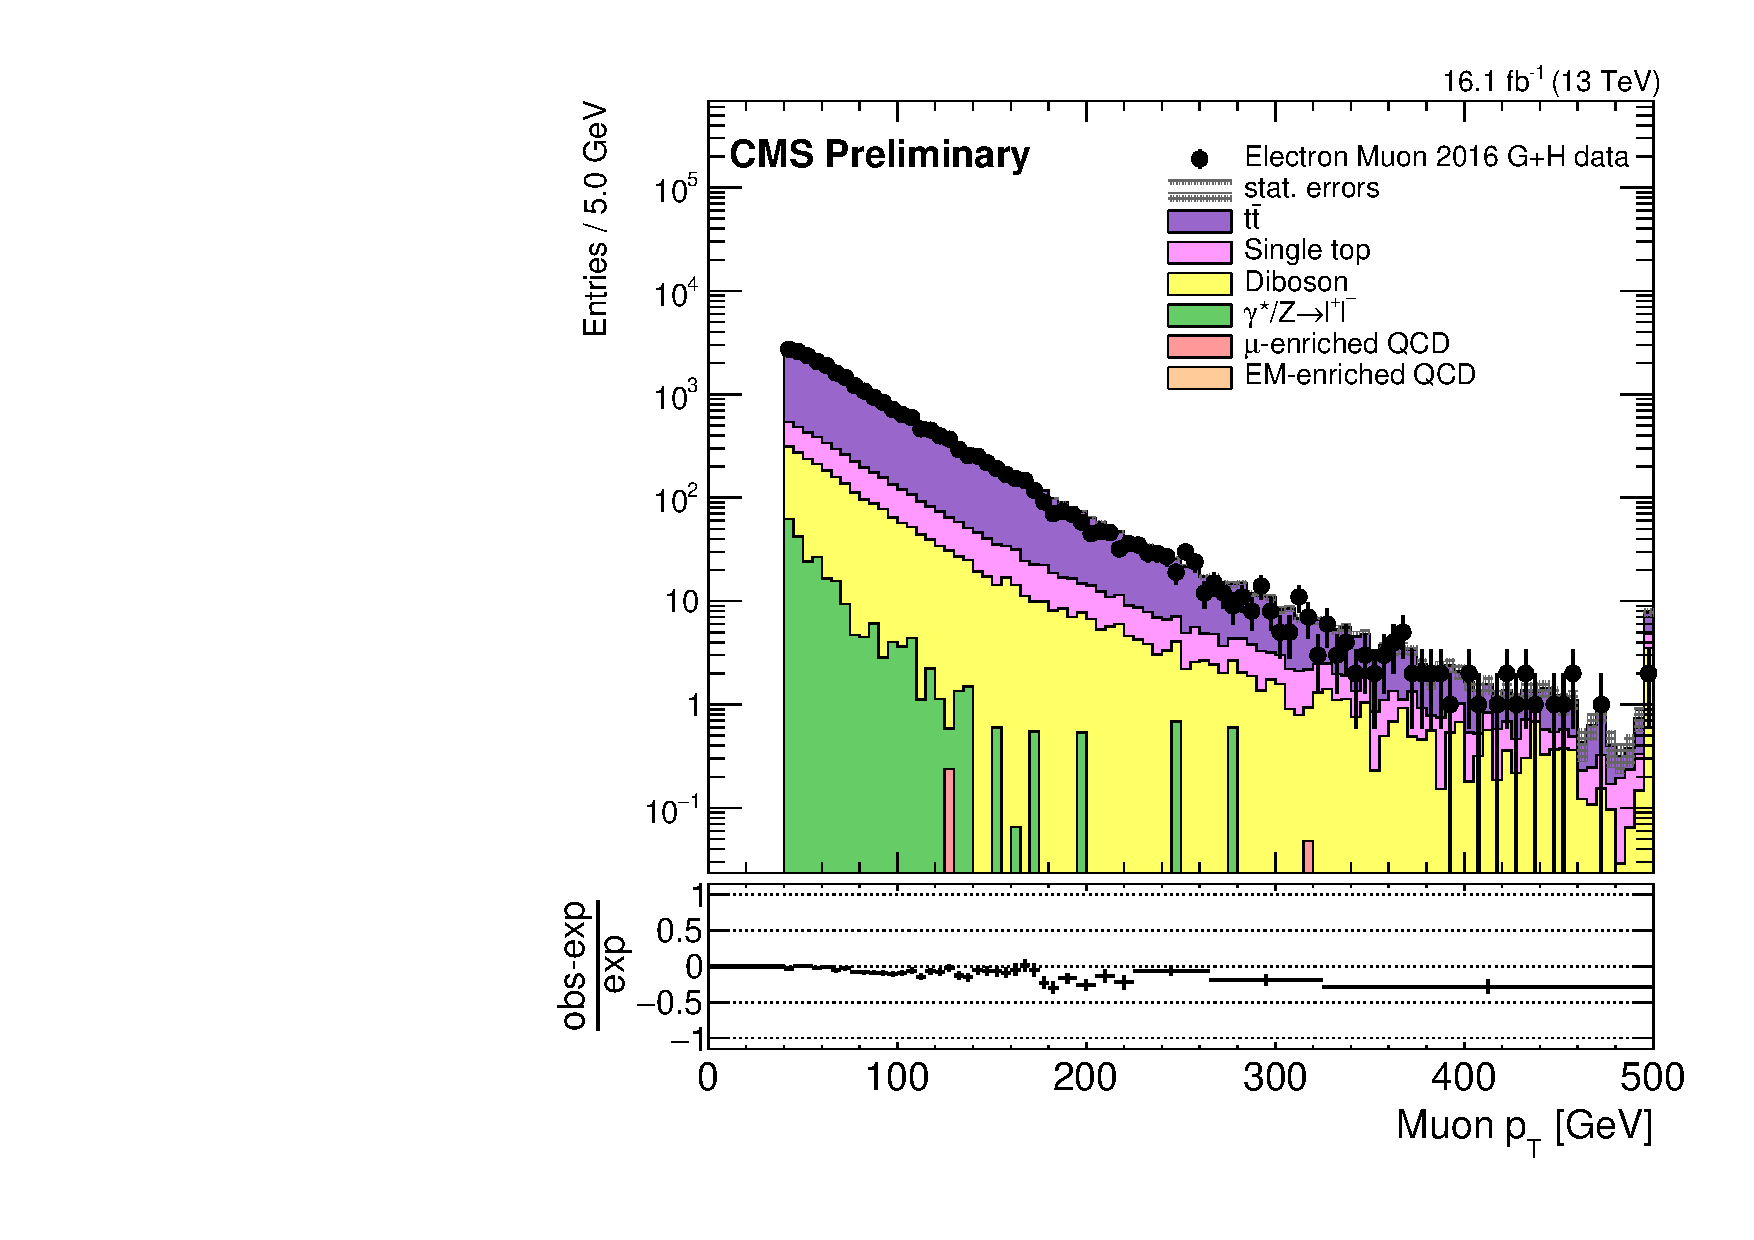
\includegraphics[width=0.3\textwidth]{figures/selection/pcr_emu_2016/muonPt.pdf}
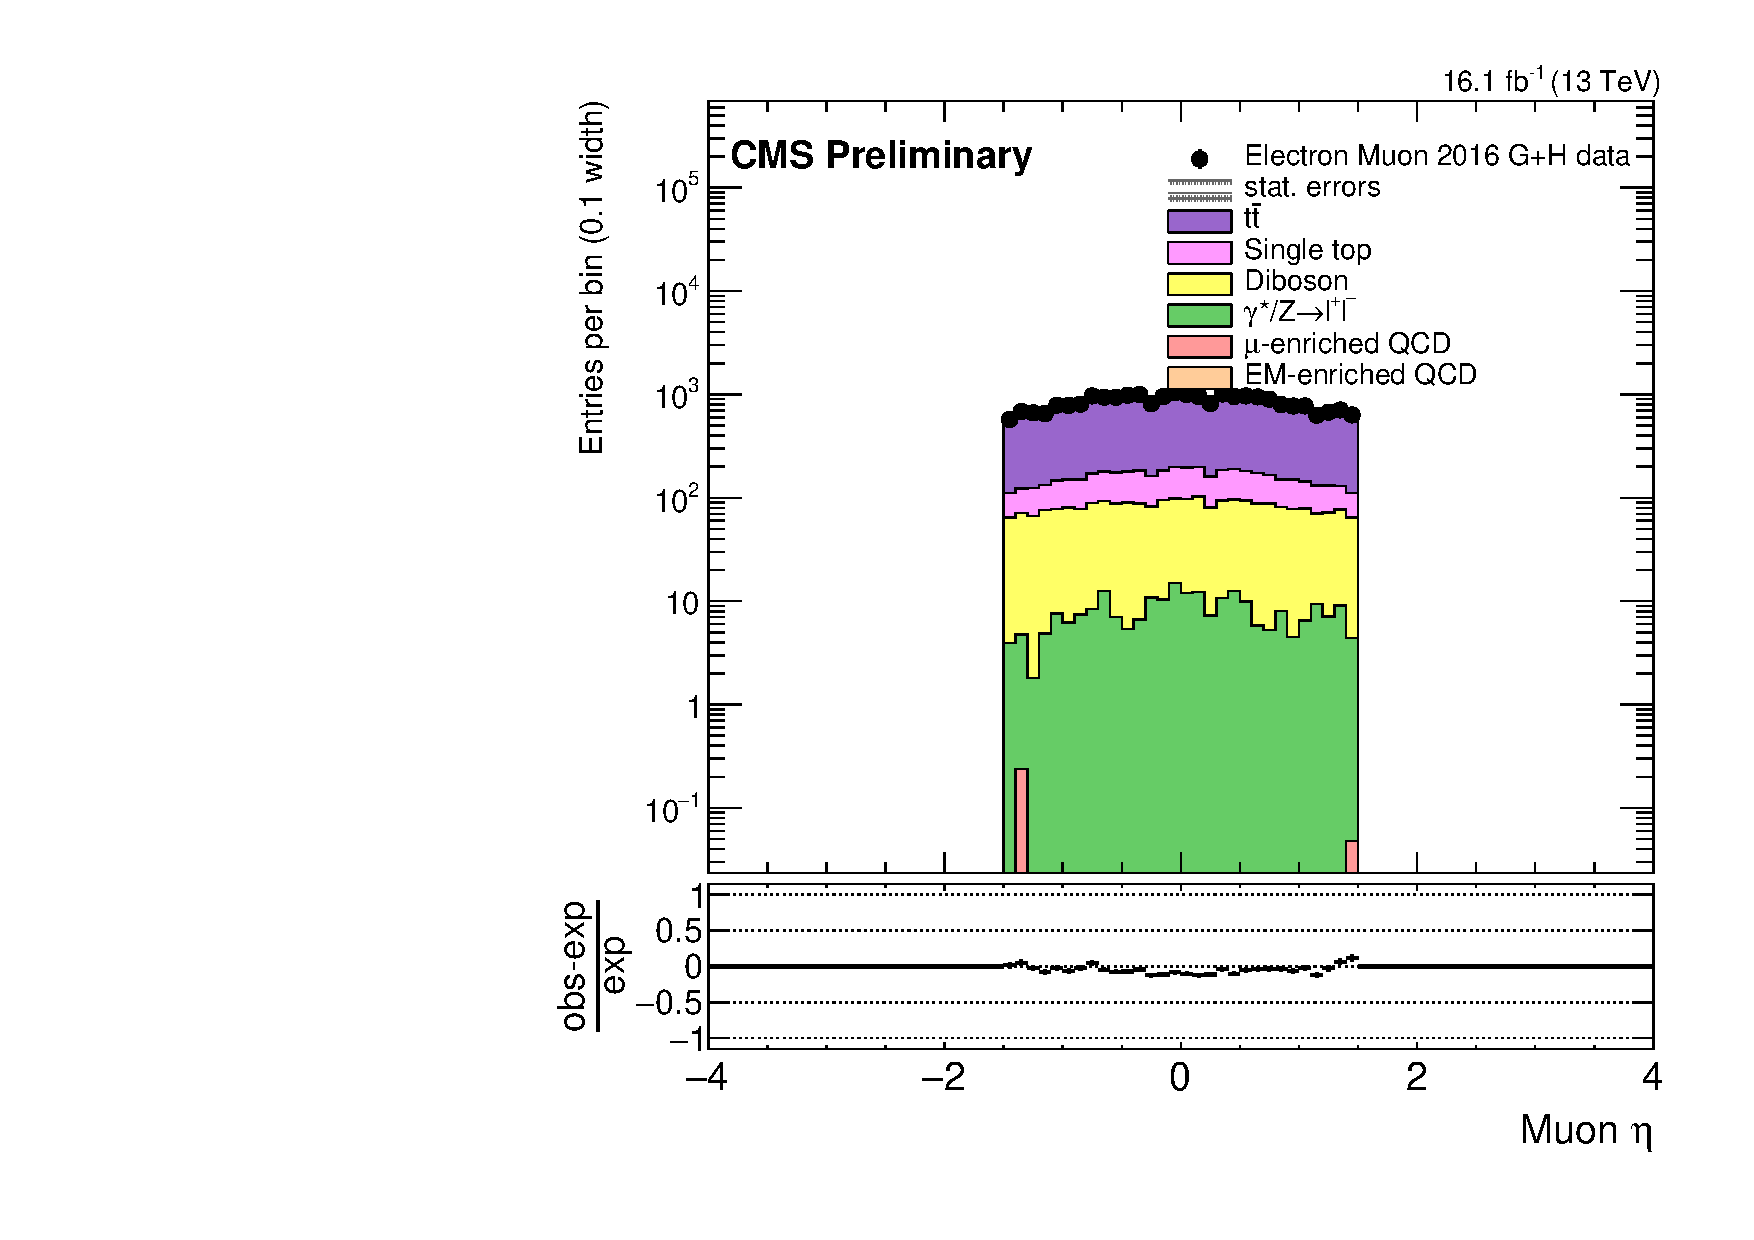
\includegraphics[width=0.3\textwidth]{figures/selection/pcr_emu_2016/muonEta.pdf}
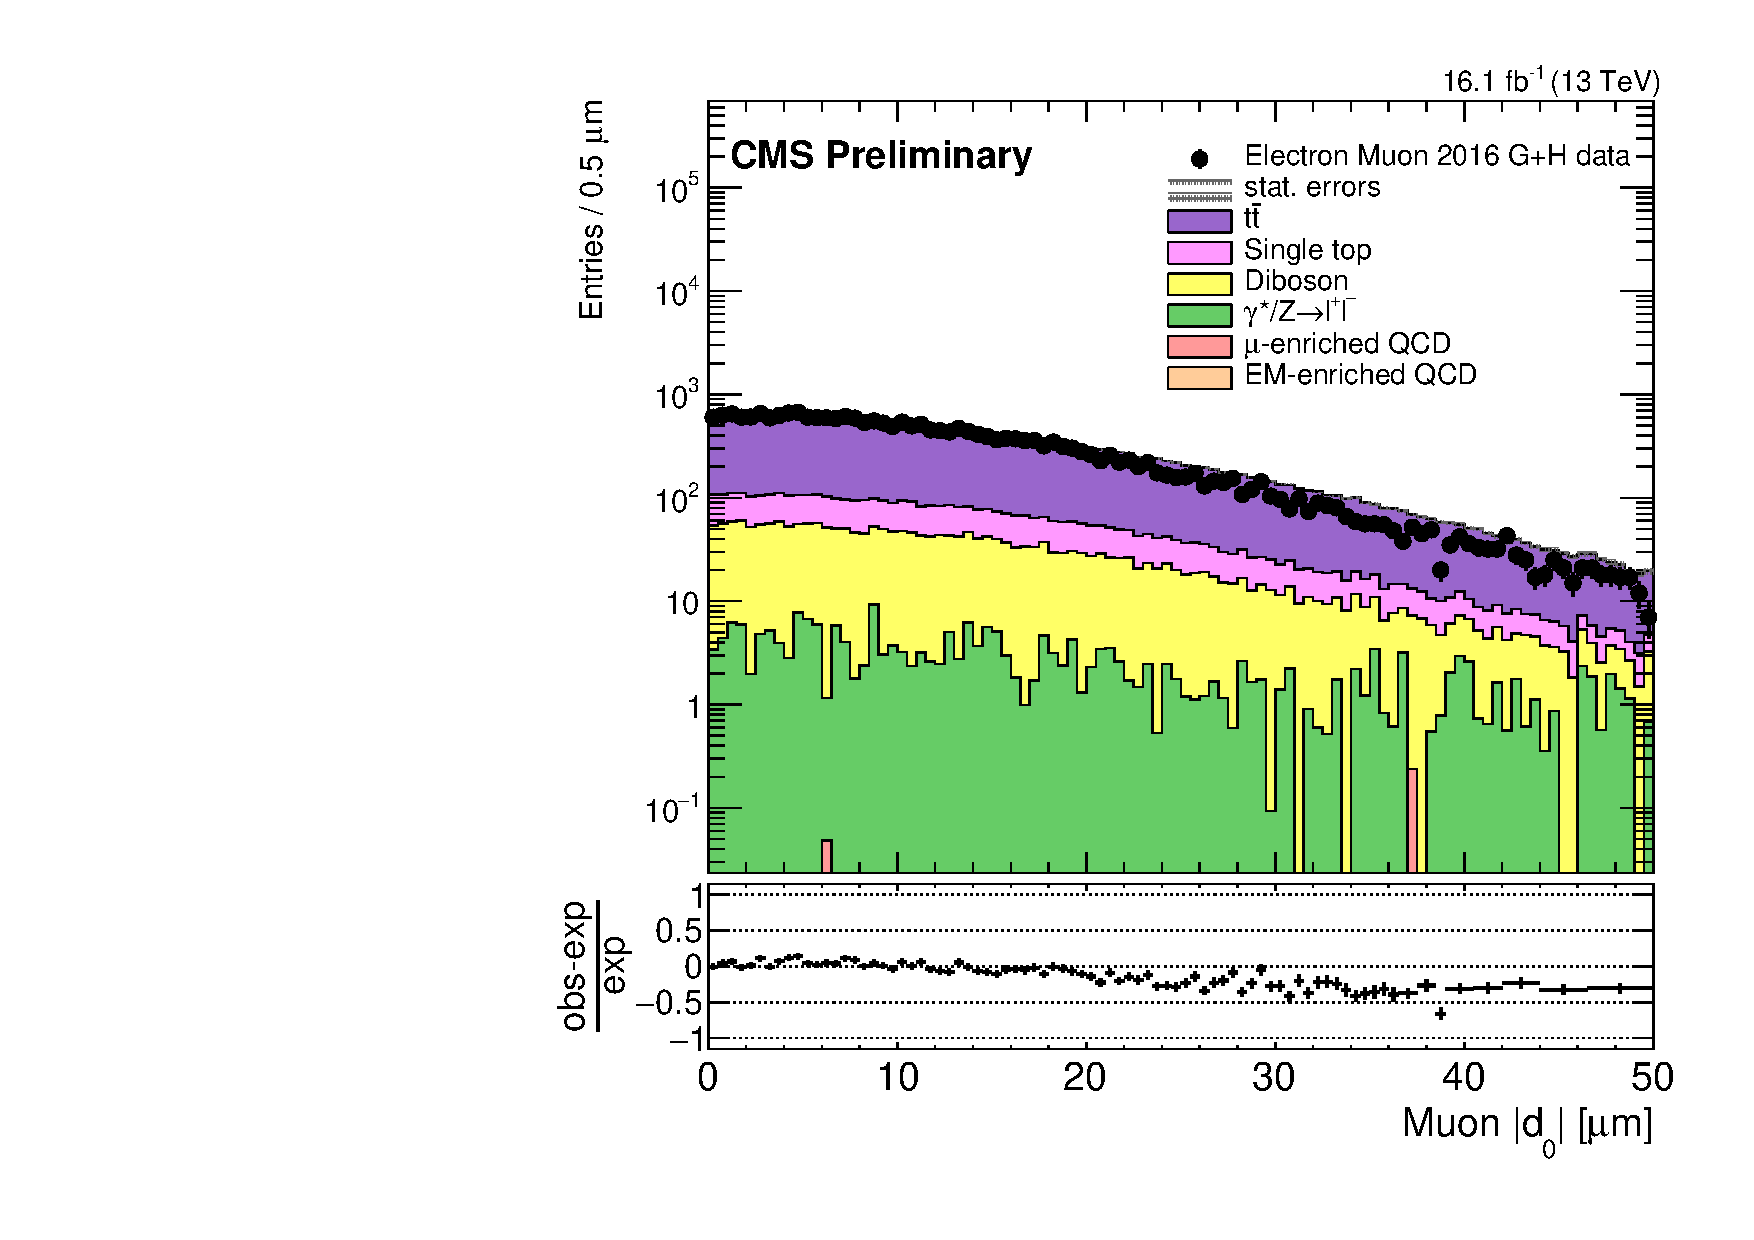
\includegraphics[width=0.3\textwidth]{figures/selection/pcr_emu_2016/muonAbsD0_50um.pdf}
\caption{The electron (top) and muon (bottom) \pt (left), $\eta$ (center), and \ad (right) distributions in the $\Pe\Pgm$ prompt control region for 2016 data and simulated background events. The rightmost bin in each plot contains the overflow entries.}
\label{pcr_emu_2016}
\end{figure}
\begin{figure}
\centering
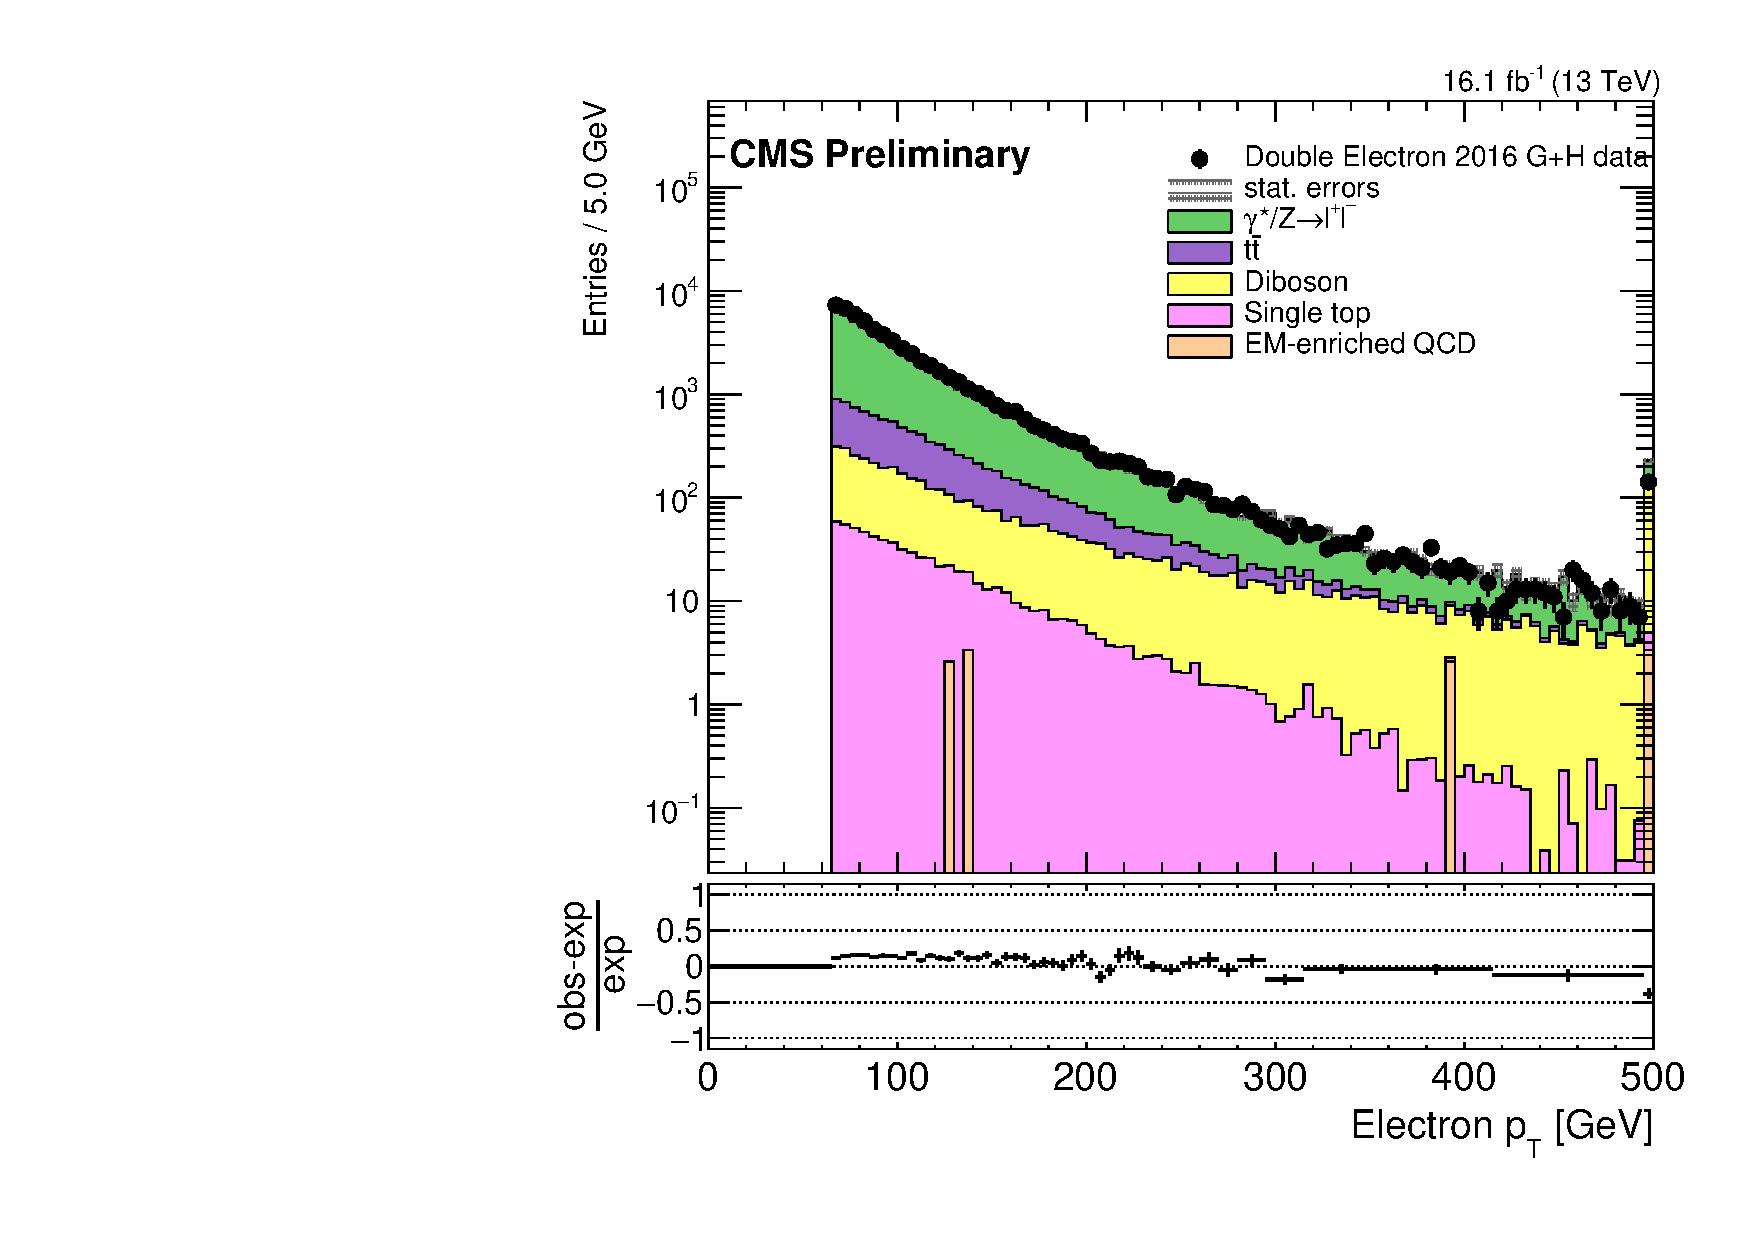
\includegraphics[width=0.3\textwidth]{figures/selection/pcr_ee_2016/electronPt.pdf}
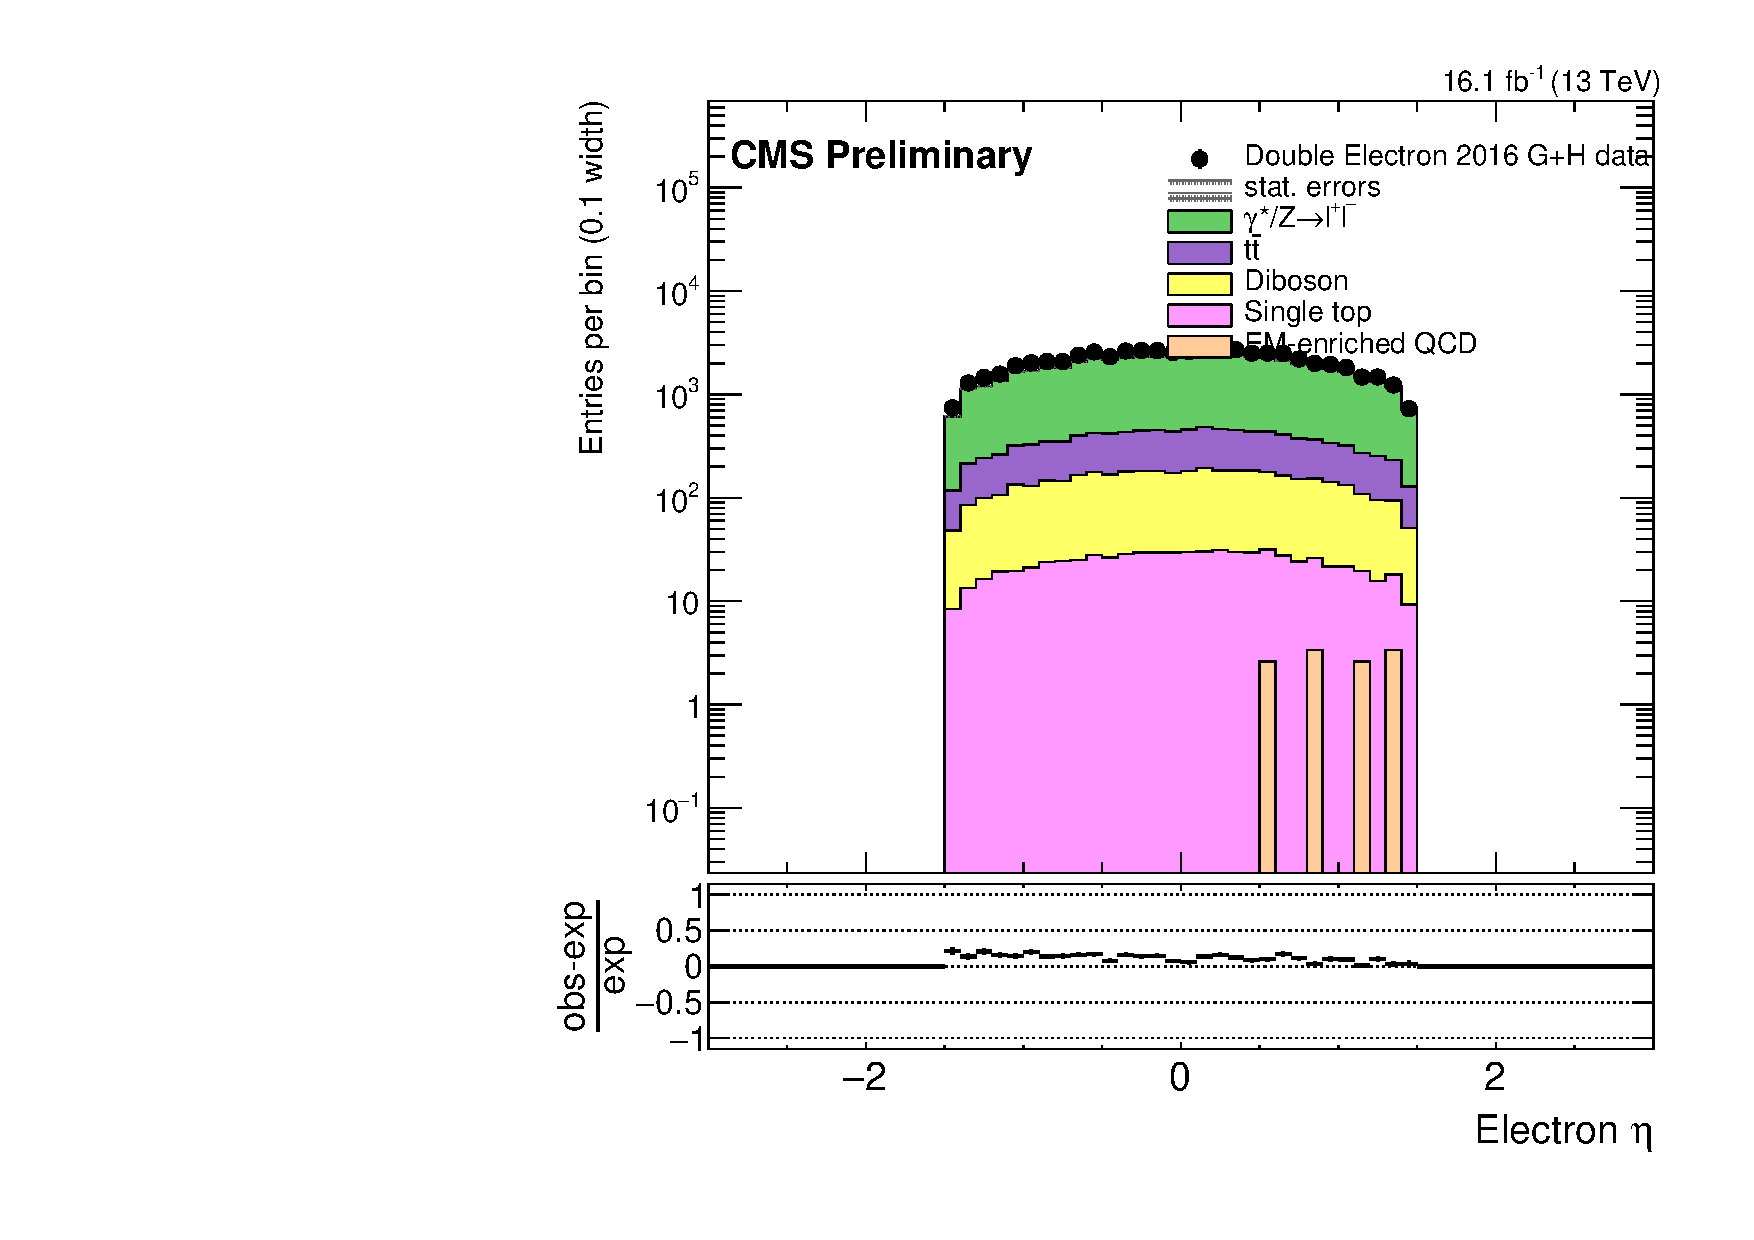
\includegraphics[width=0.3\textwidth]{figures/selection/pcr_ee_2016/electronEta.pdf}
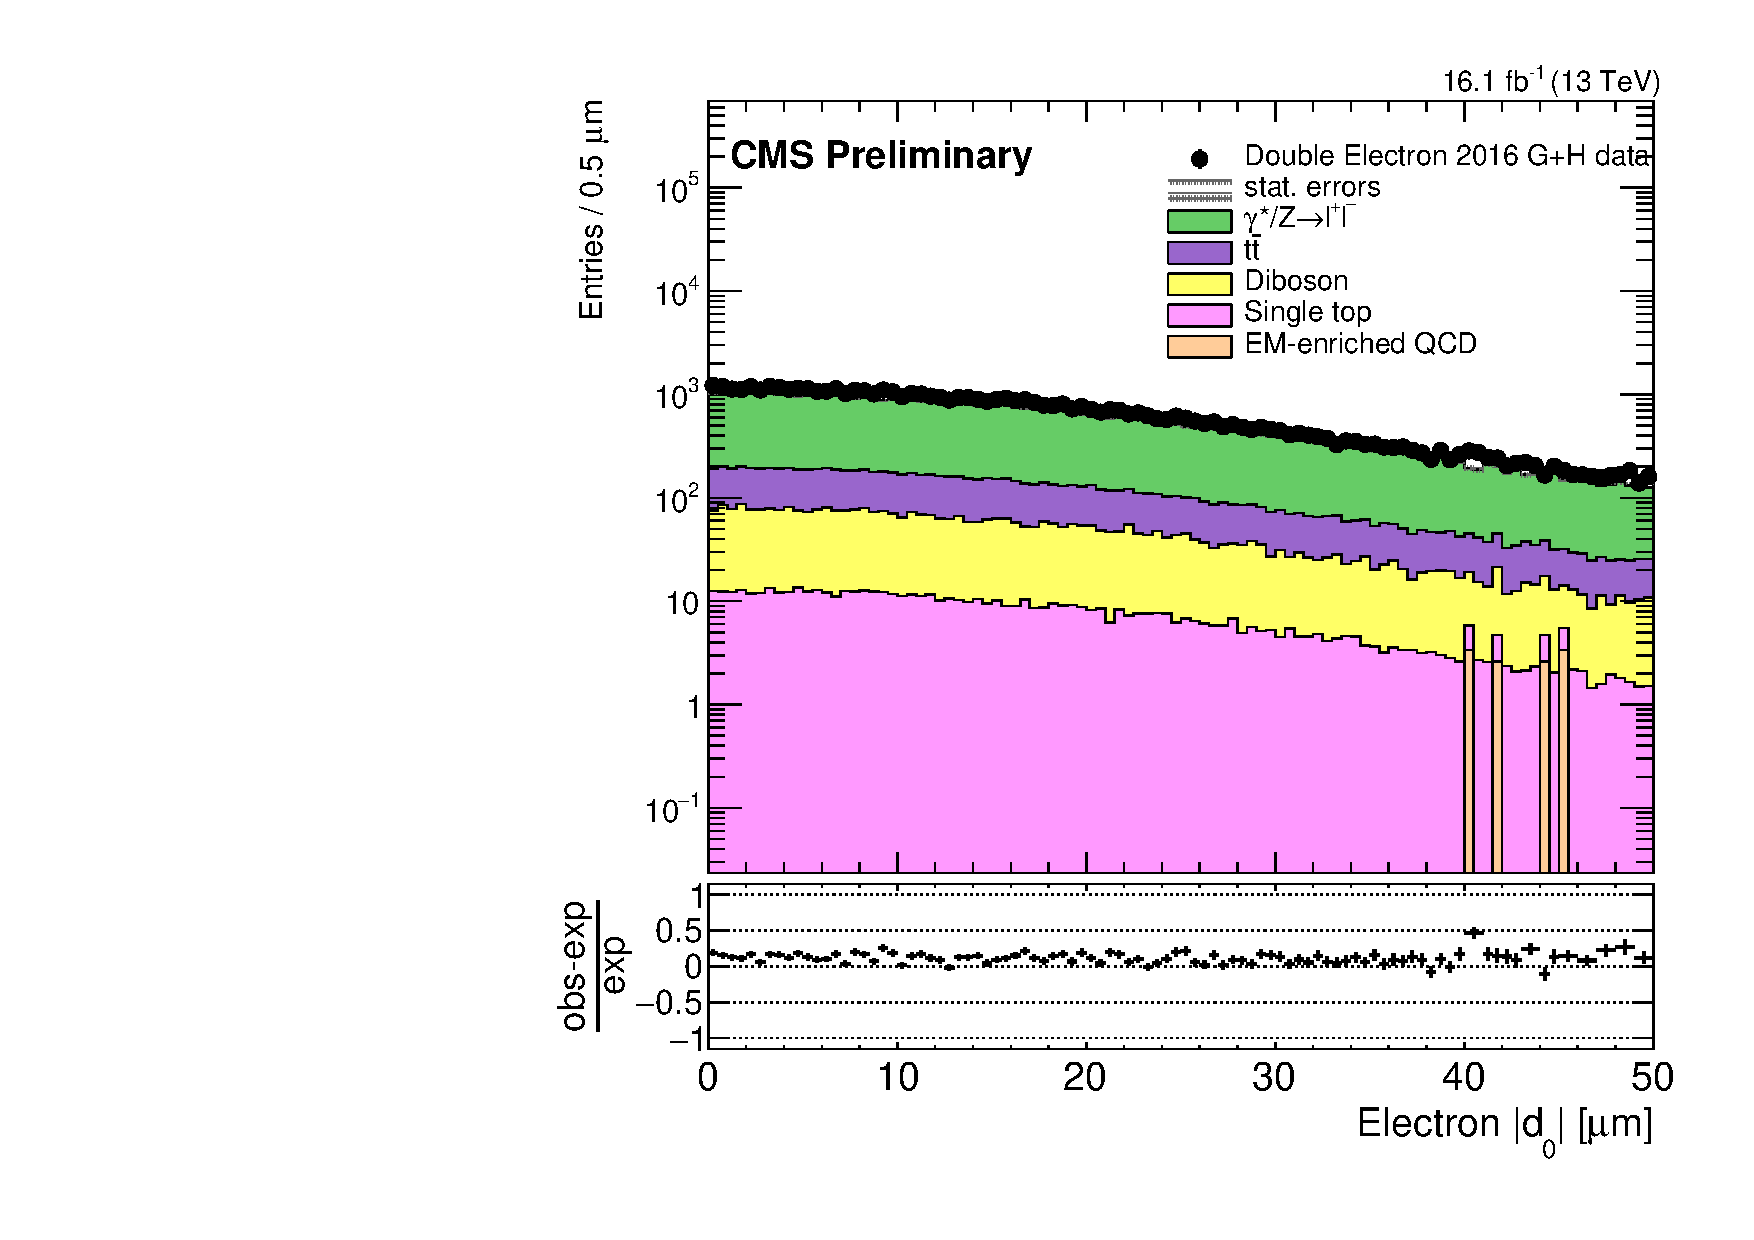
\includegraphics[width=0.3\textwidth]{figures/selection/pcr_ee_2016/electronAbsD0_50um.pdf}
\caption{The electron \pt (left), $\eta$ (center), and \ad (right) distributions in the $\Pe\Pe$ prompt control region for 2016 data and MC simulation. The rightmost bin in each plot
contains the overflow entries.}
\label{pcr_ee_2016}
\end{figure}
\begin{figure}
\centering
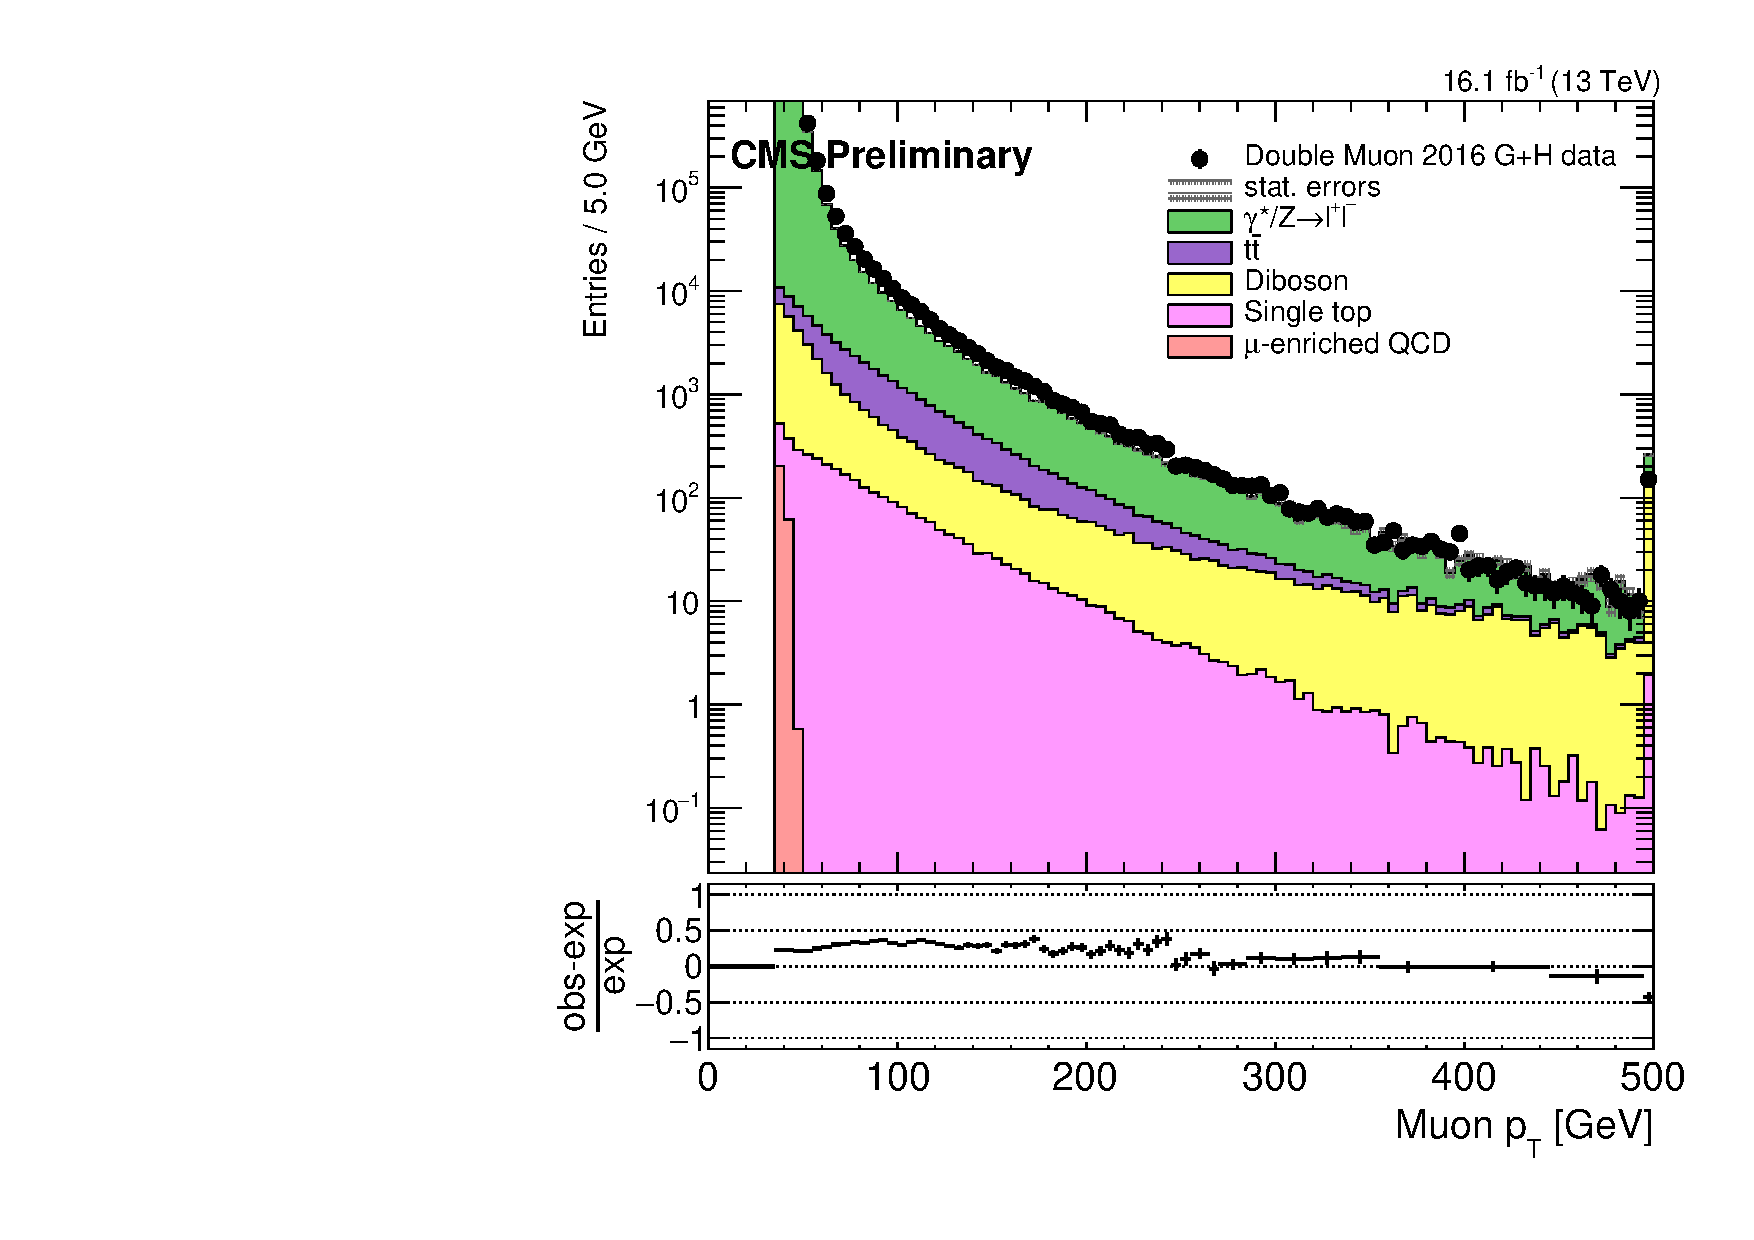
\includegraphics[width=0.3\textwidth]{figures/selection/pcr_mumu_2016/muonPt.pdf}
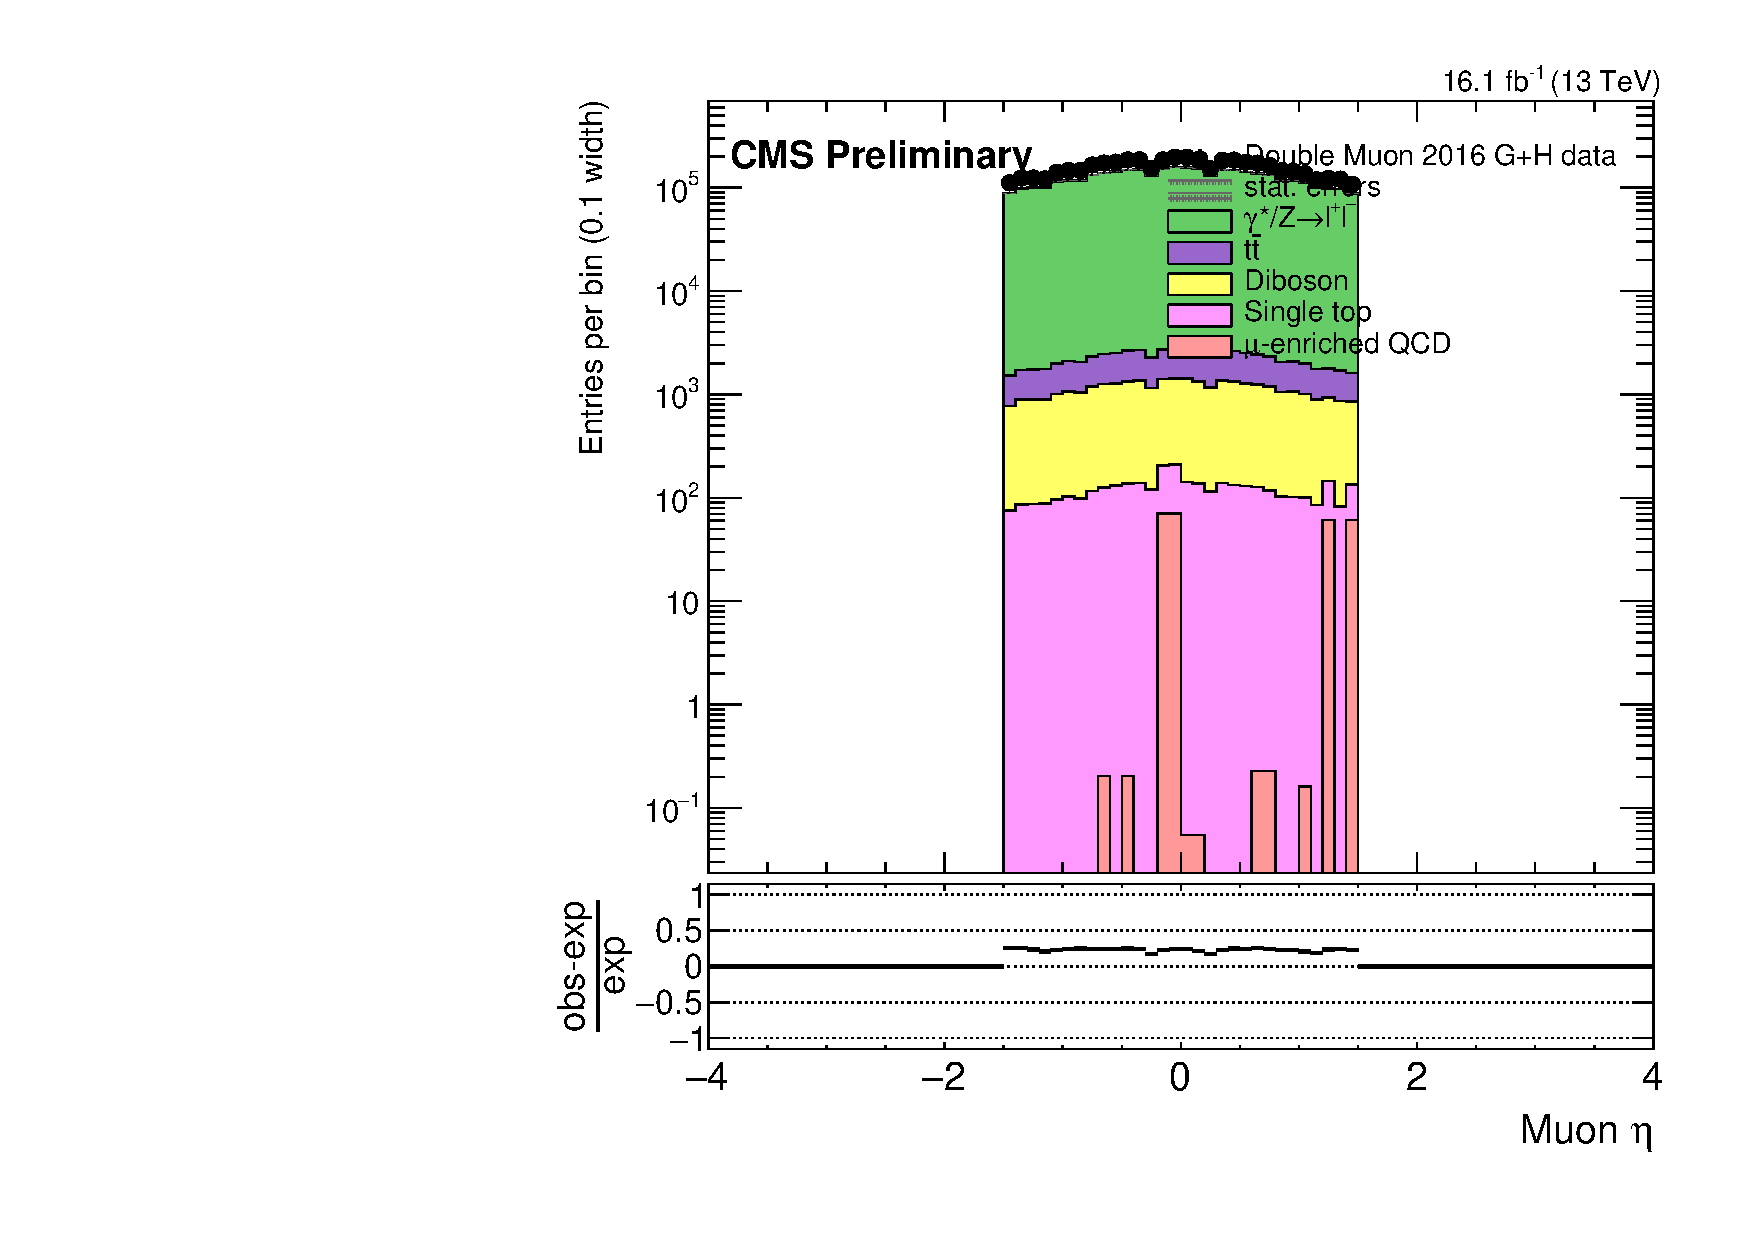
\includegraphics[width=0.3\textwidth]{figures/selection/pcr_mumu_2016/muonEta.pdf}
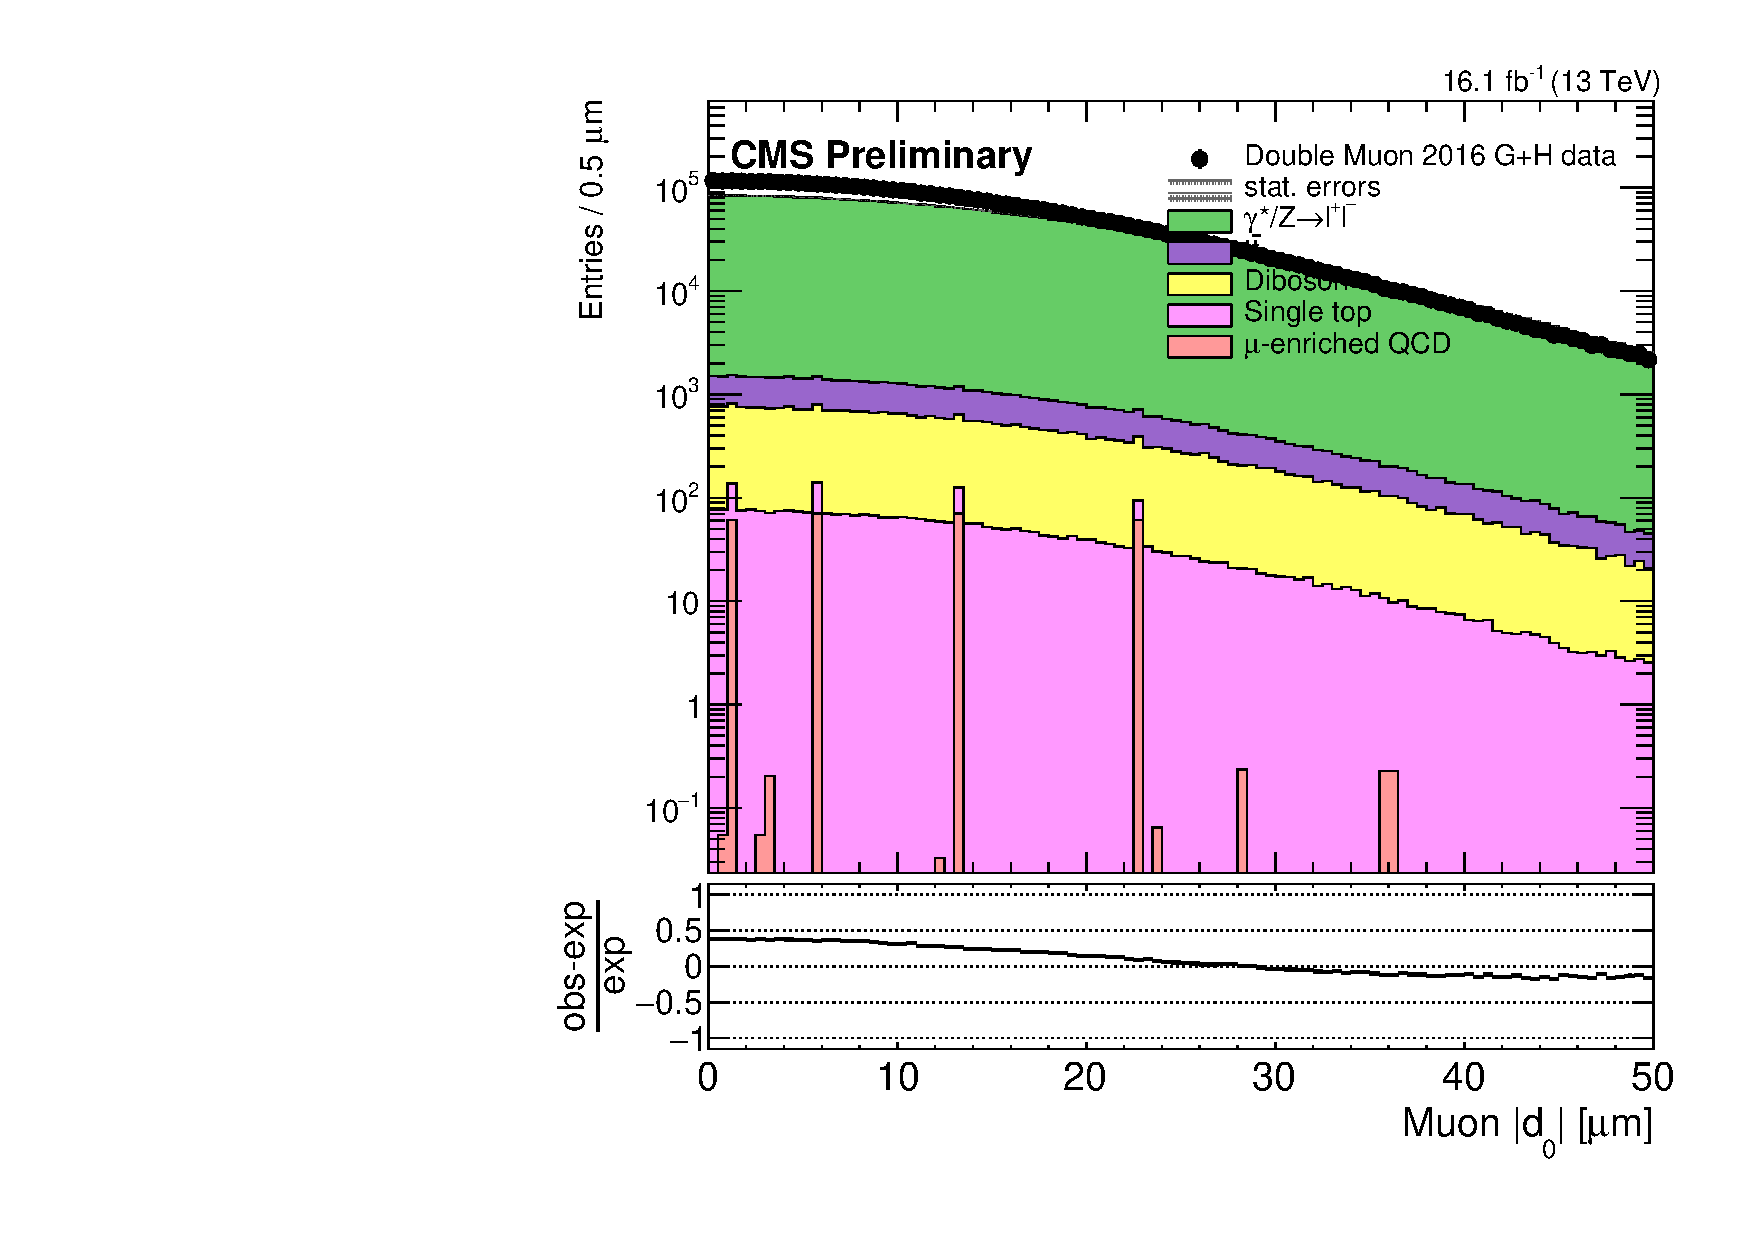
\includegraphics[width=0.3\textwidth]{figures/selection/pcr_mumu_2016/muonAbsD0_50um.pdf}
\caption{The muon \pt (left), $\eta$ (center), and \ad (right) distributions in the $\Pgm\Pgm$ prompt control region for 2016 data and MC simulation. The rightmost bin in each plot
contains the overflow entries.}
\label{pcr_mumu_2016}
\end{figure}

\subsection{Inclusive signal region}
Finally, we define inclusive signal region, which is the region in which new physics may contribute significantly. The inclusive signal region is populated by events that pass all of the criteria defined in Section~\ref{preselection} as well as the requirement that the candidate leptons each have $\SI{100}{\um}<\ad<\SI{10}{\cm}$. We do not select leptons with $\ad>\SI{10}{\cm}$ because the tracking efficiency drops sharply after this point, as shown in Section~\ref{displaced_tracking_eff}. This requirement also ensures that the leptons originate within the pixel volume, which is effectively required by the pixel hit requirement of the tight lepton IDs. To ensure sensitivity to a wide range of new particle masses and lifetimes, we further subdivide the inclusive signal region into bins defined by the \ad of each candidate lepton and the \pt of one candidate lepton. The exact binning is described in Section~\ref{abcd}.

\fxnote{it would be nice to show the d0-d0 plane somewhere here}

\pagebreak